% -*- latex -*-
\Level 0 {Introduction}

There are many ways to approach parallel programming. 
Of course you need to start with the problem that you want to solve,
but after that there can be more than one algorithm for that problem,
you may have a choice of programming systems to use
to implement that algorithm, and finally 
you have to consider the hardware that will run 
the software. Sometimes people will argue that certain problems are best solved
on certain types of hardware or with certain programming systems.
Whether this is so is indeed a question worth discussing, but 
hard to assess in all its generality.

In this tutorial we will look at one particular problem, Conway's
\emph{Game of Life}\footnote{Martin Gardner, `Mathematical Games --
  the fantastic combinations of John Conway's new solitaire game
  Life', Scientific American 223, October 1970, pp 120--123.}, and
investigate how that is best implemented using different parallel
programming systems and different hardware. That is, we will see how
different types of parallel programming can all be used to solve the
same problem.  In the process, you will learn about most of the common
parallel programming models and their characteristics.

This tutorial does not teach you to program in any particular
system: you  will only deal with \emph{pseudo-code}
and not run it on actual hardware. However, the discussion
will go into detail on the implications of using different
types of parallel computers.

(Note. At some points in this discussion there will be references to
the book `Introduction to High-Performance Scientific Computing' by
the present author\footnote
{Victor Eijkhout, with Robert van de Geijn and Edmond Chow,
  Introduction to High Performance Scientific Computing, 2011.}. Such
references take the form `HPSC-1.2.3' for section 1.2.3 of that book.)

\Level 1 {Conway's Game of Life}

The Game of Life takes place on
a two-dimensional board of \emph{cells}. Each cell can be
alive or dead, and it can switch its status from alive to dead
or the other way around once per time interval, let's say a second.
The rules for cells are as follows. In each time step, each cell
counts how many live neighbours it has, where a neighbour is a cell
that borders on it horizontallly, vertically, or diagonally. Then:
\begin{itemize}
\item If a cell is alive, and it has fewer than two live neighbours, it dies of loneliness.
\item A live cell with more than three live neighbours dies from overcrowding.
\item A live cell with two or three live neighbours lives on to the next generation.
\item A dead cell with exactly three live neighbours becomes a live cell, as if by reproduction.
\end{itemize}
The `game' is that you create an initial configuration of live cells, and then
stand back and see what happens. 
\begin{exercise}
  Here are two simple Life configurations.

  \ \hbox{
\includegraphics[scale=.2]{life-block} 
\includegraphics{life-blinker}}
  
  Go through the rules and show that the first figure is stationary,
  and the second figure morphs into something, then morphs back.
\end{exercise}
The Game of Life is hard to illustrate in a book, since it's so dynamic.
If you search online you can find some great animations.

The rules of Life are very simple, but the results can be surprising. For
instance, some simple shapes, called `gliders', seem to move over the
board; others, called `puffers', move over the board leaving behind
other groups of cells. Some configurations of cells quickly disappear,
others stay the same or alternate between a few shapes; for a~certain
type of configuration, called `garden of Eden', you can prove that it
could not have evolved from an earlier configuration. Probably most
surprisingly, Life can simulate, very slowly, a~computer!

\Level 1 {Programming the Game of Life}

It is not hard to write a program for Life. Let's say we want to compute a certain
number of time steps, and we have a square board of $N\times N$ cells.
Also assume that we have a function \n{life_evaluation} that takes a
$3\times3$ cells and returns the updated status of the center cell\footnote{We
use a quasi-python syntax here, except that in arrays we let the upper bound 
be inclusive.}:
\begin{verbatim}
def life_evaluation( cells ):
  # cells is a 3x3 array
  count = 0
  for i in [0,1,2]:
    for j in [0,1,2]:
      if i!=1 and j!=1:
        count += cells[i,j]
  return life_count_evaluation( cells[1,1],count )
def life_count_evaluation( cell,count )
  if count<2:
    return 0 # loneliness
  elif count>3:
    return 0 # overcrowding
  elif cell==1 and (count==2 or count==3):
    return 1 # live on
  elif cell==0 and count==3:
    return 1 # spontaneous generation
  else:
    return 0 # no change in dead cells
\end{verbatim}

The driver code would then be something like:
\begin{verbatim}
# create an initial board; we omit this code
life_board.create(final_time,N,N)

# now iterate a number of steps on the whole board
for t in [0:final_time-1]:
    for i in [0:N-1]:
        for j in [0:N-1]:
            life_board[t+1,i,j] = 
                life_evaluation( life_board[t,i-1:i+1,j-1:j+1] )
\end{verbatim}
where we don't worry too much about the edge of the board;
we can for instance declare that points outside the range $0\ldots N-1$ 
are always dead.

The above code creates a board for each time step, which
is not strictly necessary. You can save yourself some space
by creating only two boards:
\begin{verbatim}
life_board.create(N,N)
temp_board.create(N,N)

for t in [0:final_time-1]:
    life_generation( life_board,temp_board )

def life_generation( board,tmp ):
    for i in [0:N-1]:
        for j in [0:N-1]:
            tmp[i,j] = board[i,j]
    for i in [0:N-1]:
        for j in [0:N-1]:
            board[i,j] = life_evaluation( tmp[i-1:i+1,j-1:j+1] )
\end{verbatim}
We will call this the basic \indexterm{sequential implementation}, since it does
its computation in a long sequence of steps. We will now explore parallel
implementations of this algorithm. You'll see that some look very different 
from this basic code.

\begin{exercise}
  The second version used a whole temporary board. Can you come
  up with an implementation that uses just three temporary lines?
\end{exercise}

\Level 1 {General thoughts on parallelism}

In the rest of this tutorial we will use various types of parallelism
to explore coding the Game of Life. We start with data parallelim,
based on the observation that each point in a Life board undergoes the
same computation. Then we go on to task parallelism, which is necessary
when we start
looking at distributed memory programming on large clusters.
But first we start with some basic thoughts on parallelism.

If you're familiar with programming, you'll have read the 
above code fragments and agreed that this is a good way to 
solve the problem. You do one time step after another, and
at each time step you compute 
a new version of the board, one line after another.

Most programming languages are very explicit about loop constructs: 
one iteration is done, and then the next, and the next, and so on.
This works fine if you 
have just one processor. However, if you have some form of parallelism,
meaning that there is more than one processing unit, you have to 
figure out which things really have to be done in sequence,
and where the sequence is more an artifact of the programming language.

And by the way, \emph{you} have to think about this yourself.
In a distant past it was thought that programmers could write
ordinary code, and the compiler would figure out parallelism. This has
long proved impossible except in limited cases,
so programmers these days accept that parallel
code will look differently from sequential code, sometimes very much so.

So let's start looking at Life from a point of analyzing the parallelism.
The Life program above used three levels of loops: one for the time steps,
and two for the rows and columns of the board. While this is a correct
way of programming Life,
such explicit sequencing of loop iterations
is not strictly necessary for solving the  Game of Life problem. 
For instance,
all the cells in the new board are 
the result of independent computations, and so they
can be executed in any order, or indeed simultaneously.

You can view parallel programming as the problem of how to tell 
multiple processors that they can do certain things simultaneously,
and other things only in sequence.

\Level 0 {Parallel variants}

We will now discuss various specific parallel
realizations of Life.

\Level 1 {Data parallelism}
\label{sec:simd}

In the sequential reference code for Life we
updated the whole board in its entirety before
we proceeded to the next step. That is, we did the time steps
sequentially. 
We also observed that, in each time step, all cells can be updated
independently, and therefore in parallel. 
\begin{figure}[t]
  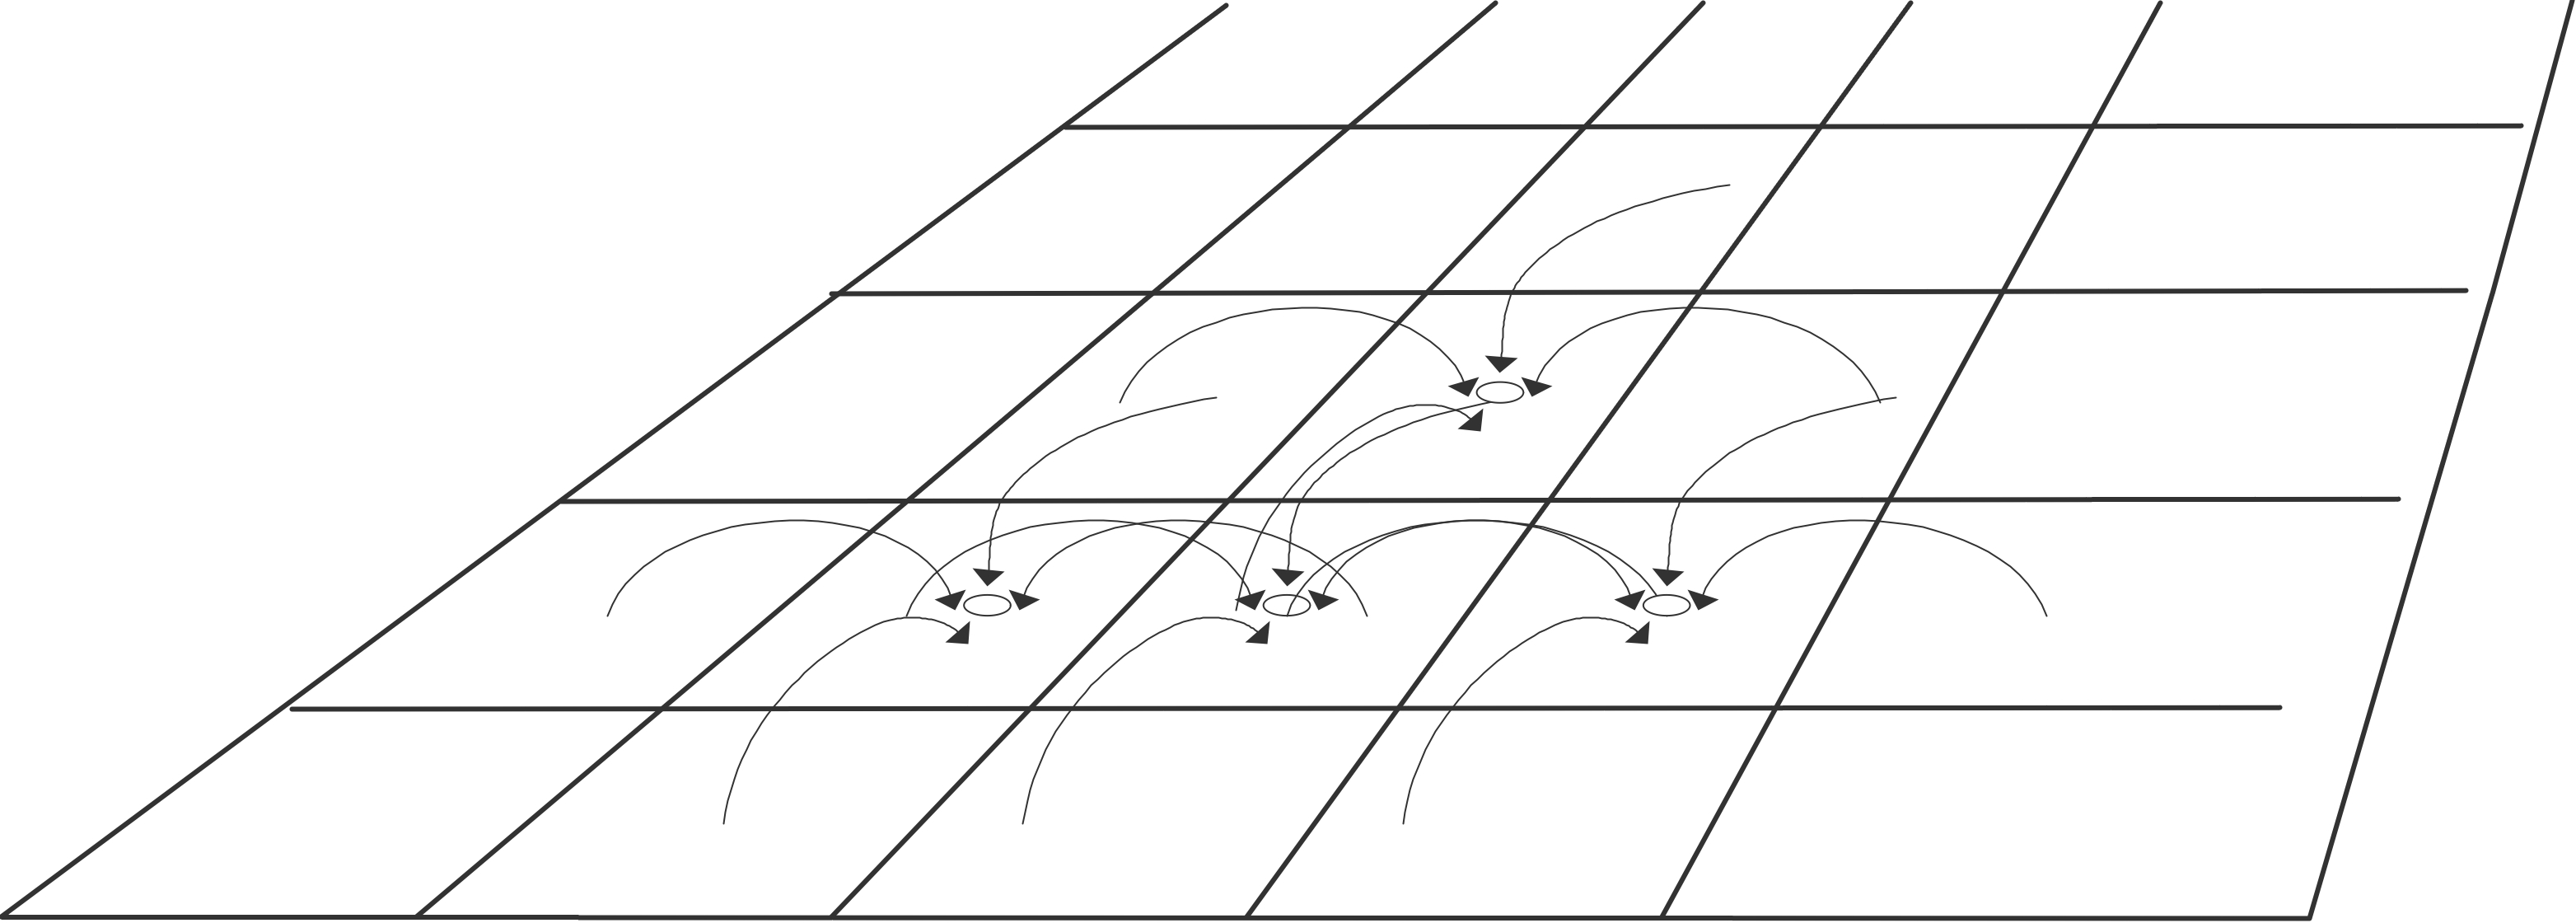
\includegraphics[scale=.1]{lifecollect}
  \caption{Illustration of data parallelism: all points of the board get the same update treatment}
  \label{fig:lifecollect}
\end{figure}
If parallelism comes in
such small chunks, we call it \indexterm{data parallelism} or
\indexterm{fine-grained parallelism}: the
parallelism comes from having lots of data points that are all treated
identically. 
This is illustrated in figure~\ref{fig:lifecollect}.

The fine-grained data parallel model of computing is known as \acf{SIMD}:
the same instruction is performed on multiple data elements.
An actual computer will of course not have an instruction for computing
a Life cell update. Rather, its instructions are things like additions and multiplications.
Thus, you may need to restructure your code a little for \ac{SIMD}
execution.

A parallel computer that is designed for doing lots of identical 
operations (on different data elements, of course) has certain advantages.
For instance, there needs to be only one central 
instruction decoding unit that tells the processors what to do,
so the design of the individual processors 
can be much simpler. This means that the processors can be smaller,
more power efficient, and easier to manufacture.

In the 1980s and 1990s \ac{SIMD} computers existed, such as the MasPar
and the Connection Machine. They were sometimes called \indexterm{array processors}
since they could operate on an array of data simultaneously,
up to $2^{16}$ elements.
These days, \ac{SIMD} still exists, but in slightly different guises
and on much smaller scale;
we will now explore what \ac{SIMD} parallelism looks like
in current architectures.

\Level 2 {Vector instructions}
\label{sec:sse}

Modern processors have embraced the \ac{SIMD} concept in an attempt to
gain performance without complicating the processor design too much.
Instead of operating on a single pair of inputs, you would load two 
or more pairs of operands,
and execute multiple identical operations simultaneously.

Vector instructions constitute \ac{SIMD} parallelism on a much smaller
scale than the old array processors. For instance, Intel processors
have had \acf{SSE} instructions for quite some time, which are
described as `two-wide' since they work on two sets of 
(double precision floating point) operands.  The
current generation of Intel vector instructions is called \acf{AVX},
and they can be up to `eight-wide'; see figure~\ref{fig:avx}
for an illustration of four-wide instructions.
\begin{figure}[t]
  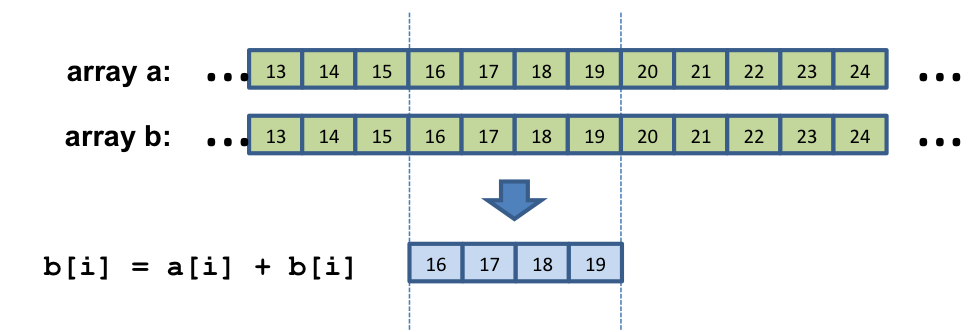
\includegraphics[scale=.7]{avx}
  \caption{Four-wide vector instructions work on four operand pairs at the same time}
  \label{fig:avx}
\end{figure}
Since with these instructions you can do four or eight operations per
clock cycle, it becomes important to write your code such that the
processor can actually use all that available parallelism.

Now suppose that you are coding the Game of Life, which is \ac{SIMD} in nature,
and you want to make sure that is executed with these vector instructions.

First of all the code needs to have the right structure. The original code
does not have a lot of parallelism in the inner loop, where it
can be exploited with vector instruction:
\begin{verbatim}
for i in [0:N]:
  for j in [0:N]:
    count = 0
    for ii in {-1,0,+1}:
      for jj in {-1,0,+1}:
        if ii!=0 and jj!=0:
          count += board[i+ii,j+jj]
\end{verbatim}
Instead, we have to exchange loops as:
\begin{verbatim}
for i in [0:N]:
  for j in [0:N]:
    count[j] = 0
  for ii in {-1,0,+1}:
    for jj in {-1,0,+1}:
      if ii!=0 and jj!=0:
        for j in [0:N]:
          count[j] += board[i+ii,j+jj]
\end{verbatim}
Note that the \n{count} variable now has become an array.
This is one of the reasons that compilers are unable to make this transformation.

Regular programming languages have no way of saying `do the following
operation with vector instructions'. That leaves you with two options:
\begin{enumerate}
\item You can start coding in assembly language, or use your
  compiler's facility for using `in-line assembly'; or
\item You can hope that the compiler understands your code enough to generate
  the vector instructions for you.
\end{enumerate}
The first option is no fun, and beyond the capabilities of most programmers,
so you'll probably rely on the compiler.

Compilers are pretty smart, but they cannot read your mind. If you code is too
sophisticated, they may not figure out that vector instructions can be used.
On the other hand, you can sometimes help the compiler. For instance,
the operation
\begin{verbatim}
for i in [0:N]:
    count[i,j] += board[i,j+1]
\end{verbatim}
can be written as
\begin{verbatim}
for ii in [0:N/2]:
    i = 2*ii
    count[i,j] += board[i,j+1]
    count[i+1,j] += board[i+1,j+1]
\end{verbatim}
Here we perform half the number of iterations, but each new iteration
comprises two old ones.
In this version the compiler will have no trouble concluding
that there are two operations that can be done simultaneously. This 
transformation of a loop is
called \indexterm{loop unrolling}, in this case, unrolling by~2.

\begin{exercise}
  The second code is not actually equivalent to the first. (Hint:
  consider the case that $N$~is odd.) How can you repair that code?
  One way of repairing this code is to add a few lines of `clean-up code'
  after the unrolled loop. Give the pseudo-code for this.

  Now consider the case of unrolling by~4. What does the unrolled code
  look like now? Think carefully about the clean-up code.
\end{exercise}

\Level 2 {Vector pipelining}
\label{sec:pipeline}

In the previous section you saw that modern CPUs can deal with
applying the same operation to a sequence of data elements.  In the
case of vector instructions (above), or in the case of GPUs (next
section), these identical operations are
actually done simultaneously. In this section we will look
at \indexterm{pipelining}, which is a different way
of dealing with identical instructions.

Imagine a car being put together on an assembly line: as the frame comes
down the line one worker puts on the wheels, another the doors,
another puts on the steering wheel, et cetera. Thus, the final
product, a car, is gradually being constructed; since more than one
car is being worked on simultaneously, this is a form of
parallelism. And while it is
possible for one worker to go through all these steps
until the car is finished, it is more efficient to let each worker
specialize in just one of the partial assembly operations.

We can do a similar story for computations in a CPU. Let's say we're
dealing with floating point numbers of the form $a.b\times 10^c$.  Now
if we add $5.8\times 10^1$ and $3.2\times 10^2$, we
\begin{enumerate}
\item first bring them to the same power of ten: $0.58\times
  10^2+3.2\times 10^2$,
\item do the addition: $3.88\times 10^2$,
\item round to get rid of that last decimal place: $3.9\times 10^2$
\end{enumerate}
So now we can apply the assembly line principle to arithmetic: 
we can let the processor do each piece in sequence, but
a~long time ago it was recognized that operations can be split up like that,
letting the sub-operations take place in different parts of the processor.
%
The processor can now work on multiple operations at the same time: we
start the first operation, and while it is under way we can start a
second one, et cetera.  In the context of computer arithmetic we call
this assembly line the \indexterm{pipeline}.

If the pipeline has four stages, after filling the pipeline there will
be four operations partially completed at any time. Thus, the pipeline
operation is roughly equivalent to, in this example, a fourfold
parallelism. You would hope that this corresponds to a fourfold speedup; 
the following exercise lets you analyze this precisely.
\begin{exercise}
  Assume that all the sub-operations take the same amount of
  time~$t$. If there are $s$ sub-operations (and
  assume~$s>\nobreak1$), how much time does it take for one full
  calculation? And how much time for two? Recognize that the time
  for two operations is less than twice the time for a single operation,
  since the second is started while the first is still in progress.

  How much time does it take to do~$n$ operations? How much
  time would $n$ operations take if the processor was not pipelined?
  What is the asymptotic improvement in speed of a pipelined processor
  over a non-pipelined one?
\end{exercise}

Around the 1970s this was the definition of a supercomputer: a machine
with a single processor that could do floating point operations
several times faster than other processors, as long as these
operations were delivered as a stream of identical operations. This
type of supercomputer essentially died out in the 1990s, but by that
time micro-processors had become so sophisticated that they started to
include pipelined arithmetic. So the idea of pipelining lives on.

Pipelining has similarities with array operations as described above:
they both apply to sequences of identical operations, and they both
apply the same operation to all operands. Because of this, pipelining
is sometimes also considered \indexac{SIMD}.

\Level 2 {GPUs}
\label{sec:gpu}

Graphics has always been an important application of computers, since
everyone likes to look at pictures. With computer games, the demand
for very fast generation of graphics has become even bigger. 
Since graphics processing is often relatively simple and structured, with 
for instance the same
blur operation executed on each pixel, or the same rendering on each polygon,
people have made specialized processors for doing just graphics. These can be
cheaper than regular processors, since they only have to do graphics-type
of operations, and they take the load off the main CPU of your computer.

Wait. Did we just say `the same operation on each pixel/polygon'? That sounds
a lot like \ac{SIMD}, and in fact it is something very close to it.

Starting from the realization that graphics processing has a lot
in common with traditional parallelism, people have tried to use \acp{GPU}
for \ac{SIMD}-type numerical computations. Doing so was cumbersome,
until \indexterm{NVIDIA} came out with the \indexacf{CUDA} language.
\ac{CUDA} is a way of explicitly doing data parallel programming:
you write a piece of code called a \indexterm{kernel}, which 
applies to a single data element. You then indicate a two-dimensional
or three-dimensional grid of points on which the kernel will be applied.

In pseudo-CUDA, a kernel definition for the game of life and its invocation
would look like:
\begin{verbatim}
kerneldef life_step( board ):
    i = my_i_number()
    j = my_j_number()
    board[i,j] = life_evaluation( board[i-1:i+1,j-1:j+1] )

for t in [0:final_time]:
    <<N,N>>life_step( board )
\end{verbatim}
where the \verb+<<N,N>>+ notation means that the processors should arrange
themselves in an $N\times N$ grid. Every processor has a way of telling
its own coordinates in that grid.

There are aspects to CUDA that make it different from SIMD, namely 
its threading, and for this reason NVIDIA uses the term
\indexacf{SIMT}.  We won't go into that here. The main purpose of this
section was to remark on the similarities between GPU programming
and \ac{SIMD} array programming.

\Level 1 {Loop-based parallelism}
\label{sec:omp}

The above strategies of parallel programming were all based on
assigning certain board locations to certain processors.
Since the locations on the board can be updated 
independently, the processors can then all work in parallel. 

There is a slightly different way of looking at this.  Rather than
going back to basics and reasoning about the problem abstractly, you
can take the code of the basic, sequential, implementation of Life.
%
Since the locations can be updated independently, the
\emph{iterations} of the loop are \emph{independent}\index{independent iterations}
and can be executed in any order, or in fact simultaneously.
So is there a way to tell the compiler that the iterations
are independent, and let the compiler decide
how to execute them?

The popular \indexterm{OpenMP} system lets the programmer
supply this information in comments:
\begin{verbatim}
def life_generation( board,tmp ):
    # OMP parallel for
    for i in [0:N-1]:
        for j in [0:N-1]:
            tmp[i,j] = board[i,j]
    # OMP parallel for
    for i in [0:N-1]:
        for j in [0:N-1]:
            board[i,j] = life_evaluation( tmp[i-1:i+1,j-1:j+1] )
\end{verbatim}
The comments here state that both
the \n{for i} loops are parallel, and
therefore their iterations can be executed by whatever parallel resources are
available.

In fact, all $N^2$ iterations of the \n{i,j} loop nest are independent,
which we express as
\begin{verbatim}
def life_generation( board,tmp ):
    # OMP parallel for collapse(2)
    for i in [0:N-1]:
        for j in [0:N-1]:
            tmp[i,j] = board[i,j]
\end{verbatim}

This approach of annotating the loops of a naively written sequential 
inplementation is a good way of getting started with parallelism.
However, the structure of the resulting parallel execution may not be
optimally suited to a given computer architecture. In the next section
we will look at different ways of getting task parallelism,
and why they may computationally be preferable.

\Level 1 {Coarse-grained data parallelism}

So far we have looked at implications of the fact that each cell in a
step of Life can be updated independently. This view leads to tiny grains
of computing, which are a good match to the innermost components of
a processor core. However, if you look at parallelism on the level
of the cores of a processor there are disadvantages to 
assigning small-grained computations randomly to the cores. 
Most of these have something to do with the way memory is structured:
moving such small amounts of work around can be more costly
than executing them
(for a detailed discussion see section~\HPSCref{sec:hierarchy}).
Therefore, we are motivated to look at computations in 
larger chunks than  a single cell
update. 

For instance, we can divide the Life board in lines or square patches,
and formulate the algorithm in terms of operations on such larger units.
This is called \indexterm{coarse-grained parallelism}, and we will look
at several variants of it.

\Level 2 {Shared memory parallelism}
\label{sec:shared}

In the approaches to parallelism mentioned so far we have 
implicitly assumed that a processing element can actually get hold of any data
element it needs. Or look at it this way: a~program has a set of instructions
and so far we have assumed that any processor can execute any instruction.

This is certainly the case with multicore processors,
where all cores can equally easily read any element from memory.
\begin{figure}[t]
  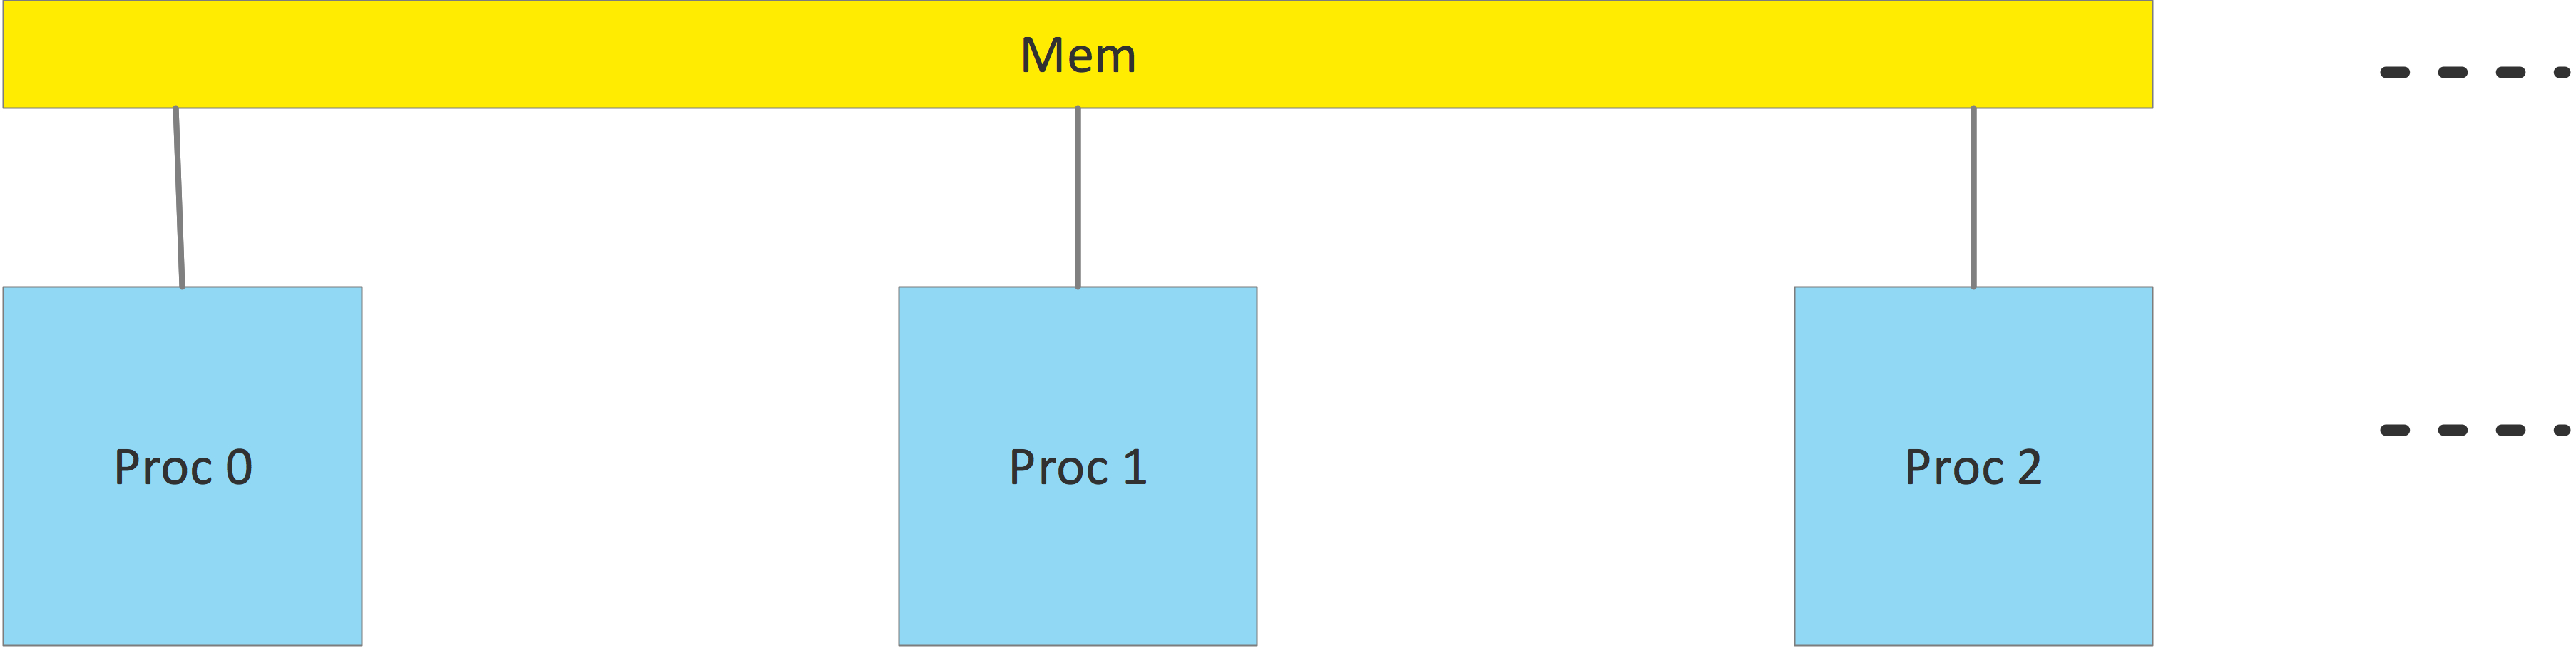
\includegraphics[scale=.1]{shared}
  \caption{Illustration of shared memory: all processors access the
    same memory}
  \label{fig:shared}
\end{figure}
We call this \indextermsub{shared}{memory}; see figure~\ref{fig:shared}.

In the CUDA example each
processing element essentially reasoned `this is my number, and
therefore I~will work on this element of the array'. 
In other words, each processing element assumes that it can 
work on any data element, and this works
because a GPU has a form of shared memory.

While it is convenient to program this way, it is not possible to make
arbitrarily large computers with shared memory.
The shared memory approaches discussed so far are limited by the
amount of memory you can put in a single PC, at the moment about
1~terabyte (which costs a lot of money!), or the processing power
that you can associate with shared memory, at the moment around
48~cores.

If you need more processing power, you need to look at clusters,
and `distributed memory programming'.

\Level 2 {Distributed memory parallelism}
\label{sec:spmd}

\begin{figure}[t]
  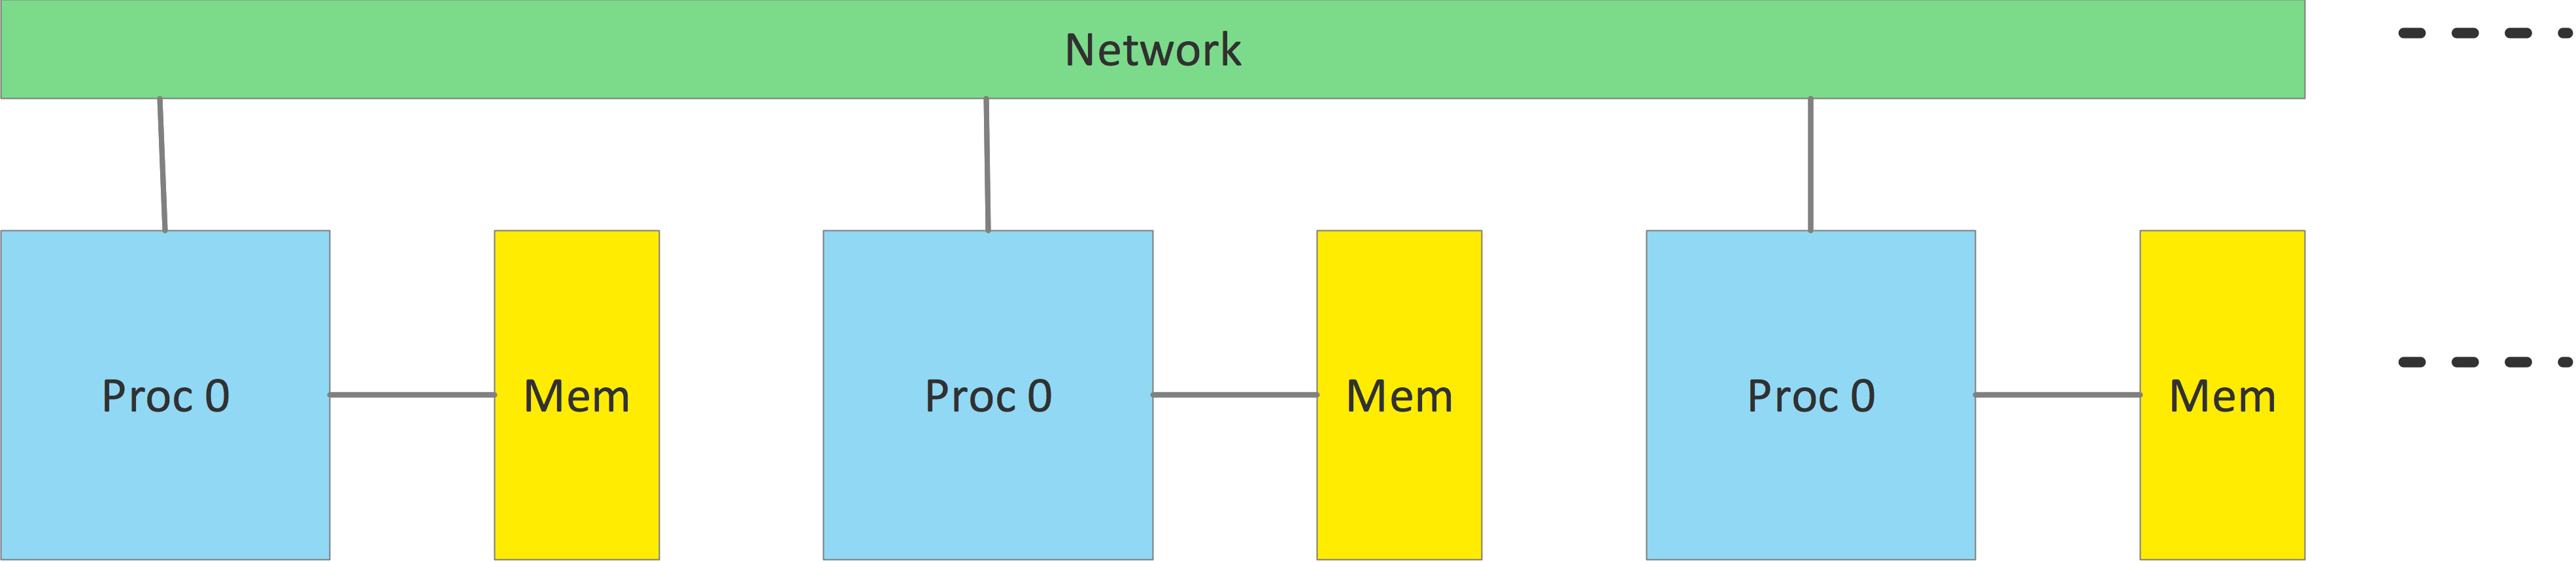
\includegraphics[scale=.1]{distributed}
  \caption{Illustration of distributed memory: every processor has its
    own memory and is connected to others through a network}
  \label{fig:spmd}
\end{figure}

\emph{Clusters}\index{clusters},
also called \indextermsub{distributed}{memory} computers,
can be thought of
as a large number of PCs with network cabling between them.
This design can be scaled up to a much larger number of processors
than shared memory.
In the context of a cluster, each of these PCs
is called a \indexterm{node}. The network can be
\indexterm{Ethernet} or something more sophisticated like \indexterm{Infiniband}.

Since all nodes work together, a~cluster is in some sense one
large computer. 
Since the nodes are also to an extent independent, this type of parallelism is
called \indexacf{MIMD}: each node has its own data, and executes its own program.
However, most of the time the nodes will all execute
the same program, so this model is often called \indexacf{SPMD}; see figure~\ref{fig:spmd}.
The advantage of this design is that tying
together thousands of processors allows you to run very large problems.
For instance, the almost 13 thousand processors of the Stampede supercomputer\footnote
{Stampede has more than 6400 nodes, each with 2 Intel Sandy Bridge processors.
Each node also has an Intel Xeon Phi co-processor, but we don't count those for the moment.}
\begin{figure}[t]
  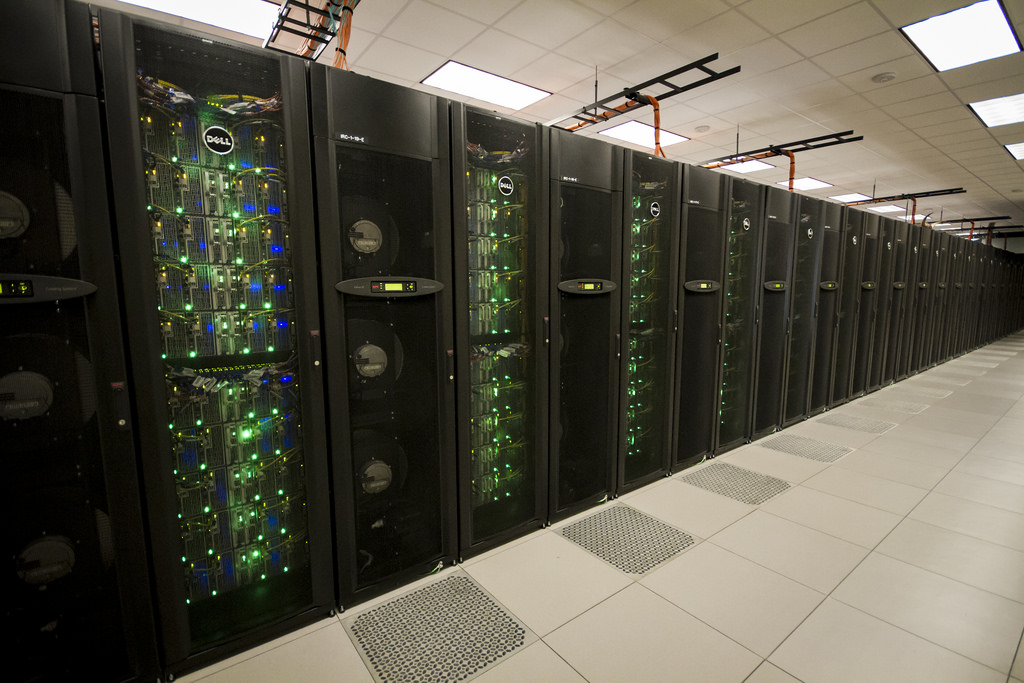
\includegraphics[scale=.75]{stampede-cable}
  \caption{The Stampede supercomputer at the Texas Advanced Supercomputing Center}
  \label{fig:stampede}
\end{figure}
(figure~\ref{fig:stampede}) have almost 200 terabytes of memory.
Parallel programming on such a machine is a little harder
than what we discussed above.
First of all we have to worry about
how to partition the problem over this \indexterm{distributed memory}.
But more importantly, our above assumption that each processing element
can get hold of every data element no longer holds.

It is clear that each cluster node can access its local
problem data without any problem, but this is not true for the `remote' data
on other nodes.
In the former case the program simply reads the memory location;
in the latter case accessing data is only possible because there is a network
between the processors: in the Stampede picture you can see yellow cabling
connecting the nodes in each cabinet, and orange cabling overhead that connects the cabinets.
Accessing data over the network
probably involves an operating system call and accessing
the network card, both of which are slow operations.

\Level 2 {Distributed memory programming}
\label{sec:mpi}

By far the most popular way for programming distributed memory
machines is by using the \acf{MPI} library. This library adds
functionality to an otherwise normal C~or~Fortran program for
exchanging data with other processors. The name derives
from the fact that the technical term for
exchanging data between distributed memory nodes
is \indexterm{message passing}.

Let's explore how you would program with MPI.
We start with the case that each processor stores the cells
of a single line of the Life board, and that processor~$p$ stores line~$p$.
In that case, to update that line
it needs the lines above and below it, which come from processors $p-1$ and $p+1$
respectively. In MPI terms, the processor needs to receive a message
from each of these processors, containing the state of their line.

Let's build up the basic structure of an MPI program. 
Througout this example, keep in mind that we are working in \ac{SPMD} mode:
all processes execute the same program.
As illustrated in figure~\ref{fig:mpiget}
\begin{figure}[t]
  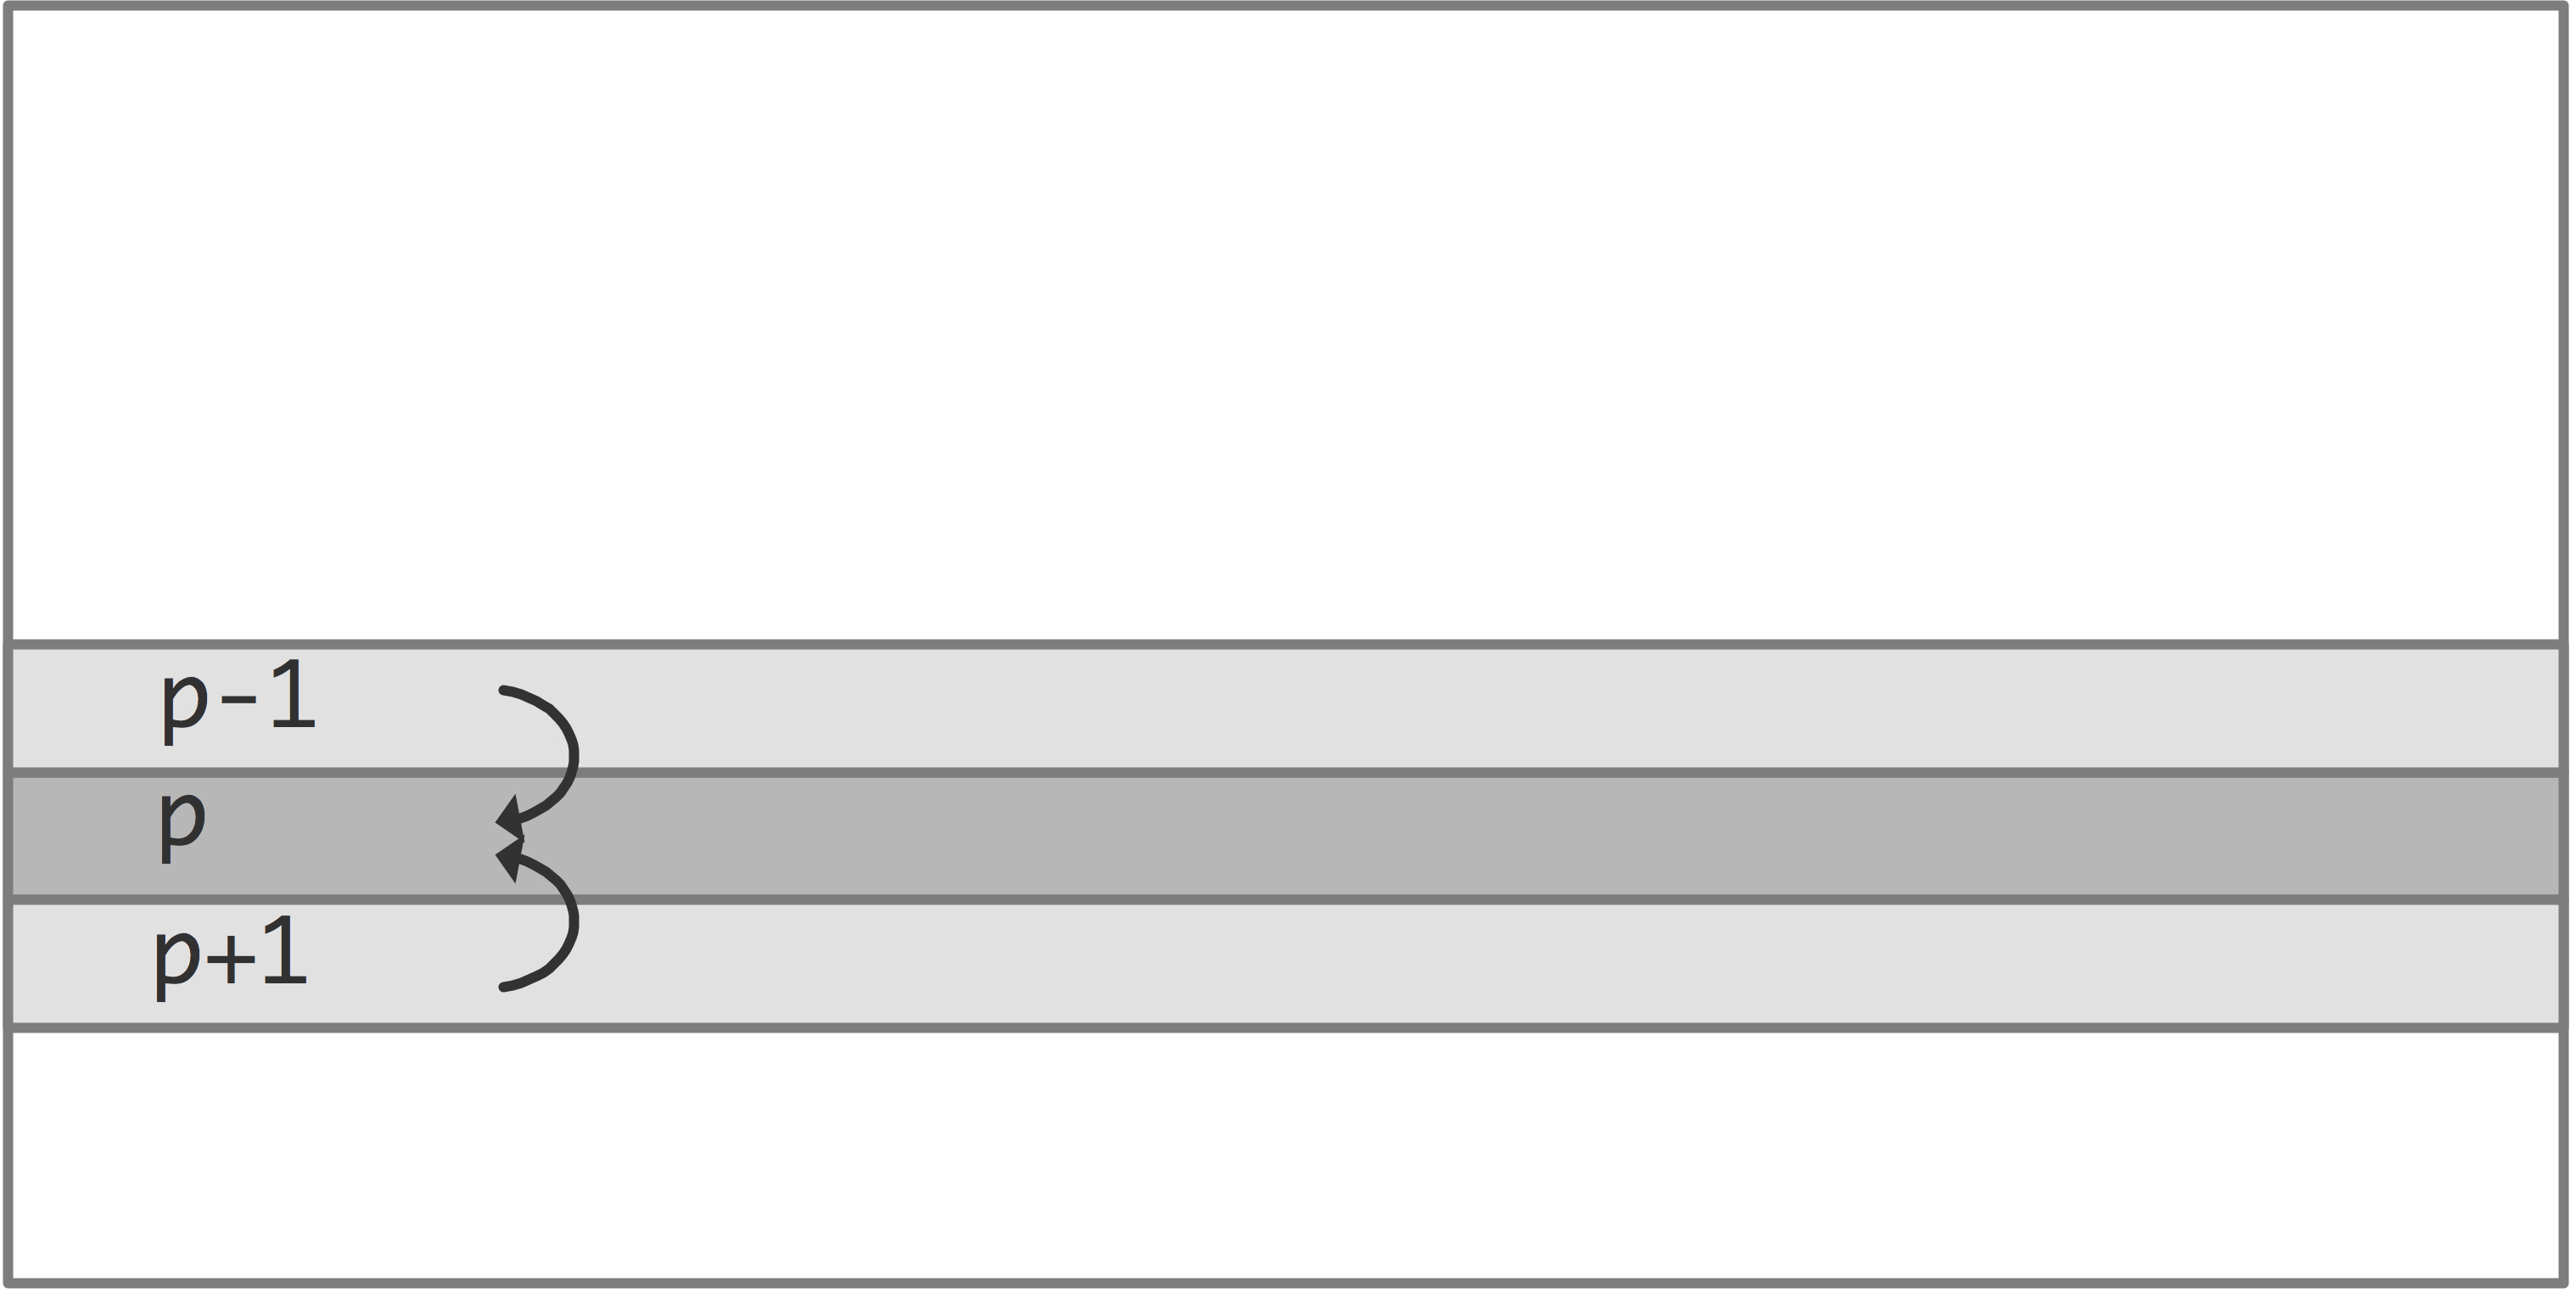
\includegraphics[scale=.1]{mpiget}
  \caption{Processor $p$ receives a line of data from $p-1$ and $p+1$}
  \label{fig:mpiget}
\end{figure}
a process needs to get data from its neighbours. 
The first step is for each process to find out what its number is,
so that it can name its neigbours.
\begin{verbatim}
p = my_processor_number()
\end{verbatim}
Then the process can actually receive data from those neighbours
(we ignore complications from the first and last line of the board here).
\begin{verbatim}
high_line = MPI_Receive(from=p-1,cells=N)
low_line = MPI_Receive(from=p+1,cells=N)
\end{verbatim}
With this, it is possible to update the data stored on this process:
\begin{verbatim}
tmp_line = my_line.copy()
my_line = life_line_update(high_line,tmp_line,low_line,N)
\end{verbatim}
(We omit the code for \n{life_line_update}, which computes the updated
cell values on a single line.)
Unfortunately, there is more to MPI than that. The most common way
of using the library is through \indextermsub{two-sided}{communication},
where for each receive action there is a corresponding send action:
a~process cannot just receive data from its neighbours, the neighbours
have to send the data.

But now we recall the \ac{SPMD} nature of the computation: 
if your neighbours send to you, you are someone else's neighbour and
need to send to them. So the program code will contain both
send and receive calls.

The following code is closer to the truth.
\begin{verbatim}
p = my_processor_number()

# send my data
my_line.MPI_Send(to=p-1,cells=N)
my_line.MPI_Send(to=p+1,cells=N)

# get data from neighbours
high_line = MPI_Receive(from=p-1,cells=N)
low_line = MPI_Receive(from=p+1,cells=N)
tmp_line = my_line.copy()

# do the local computation
my_line = life_line_update(high_line,tmp_line,low_line,N)
\end{verbatim}
Since this is a general tutorial, and not a course in MPI programming,
we'll leave the example phrased in pseudo-MPI, ignoring many details.
However, this code is still not entirely
correct conceptually. Let's fix that.

Conceptually, a process would send a message, which disappears
somewhere in the network, and goes about its business.
The receiving process would at some point issue a receive call,
get the data from the network, and do something with it.
\begin{figure}[t]
  \leavevmode
  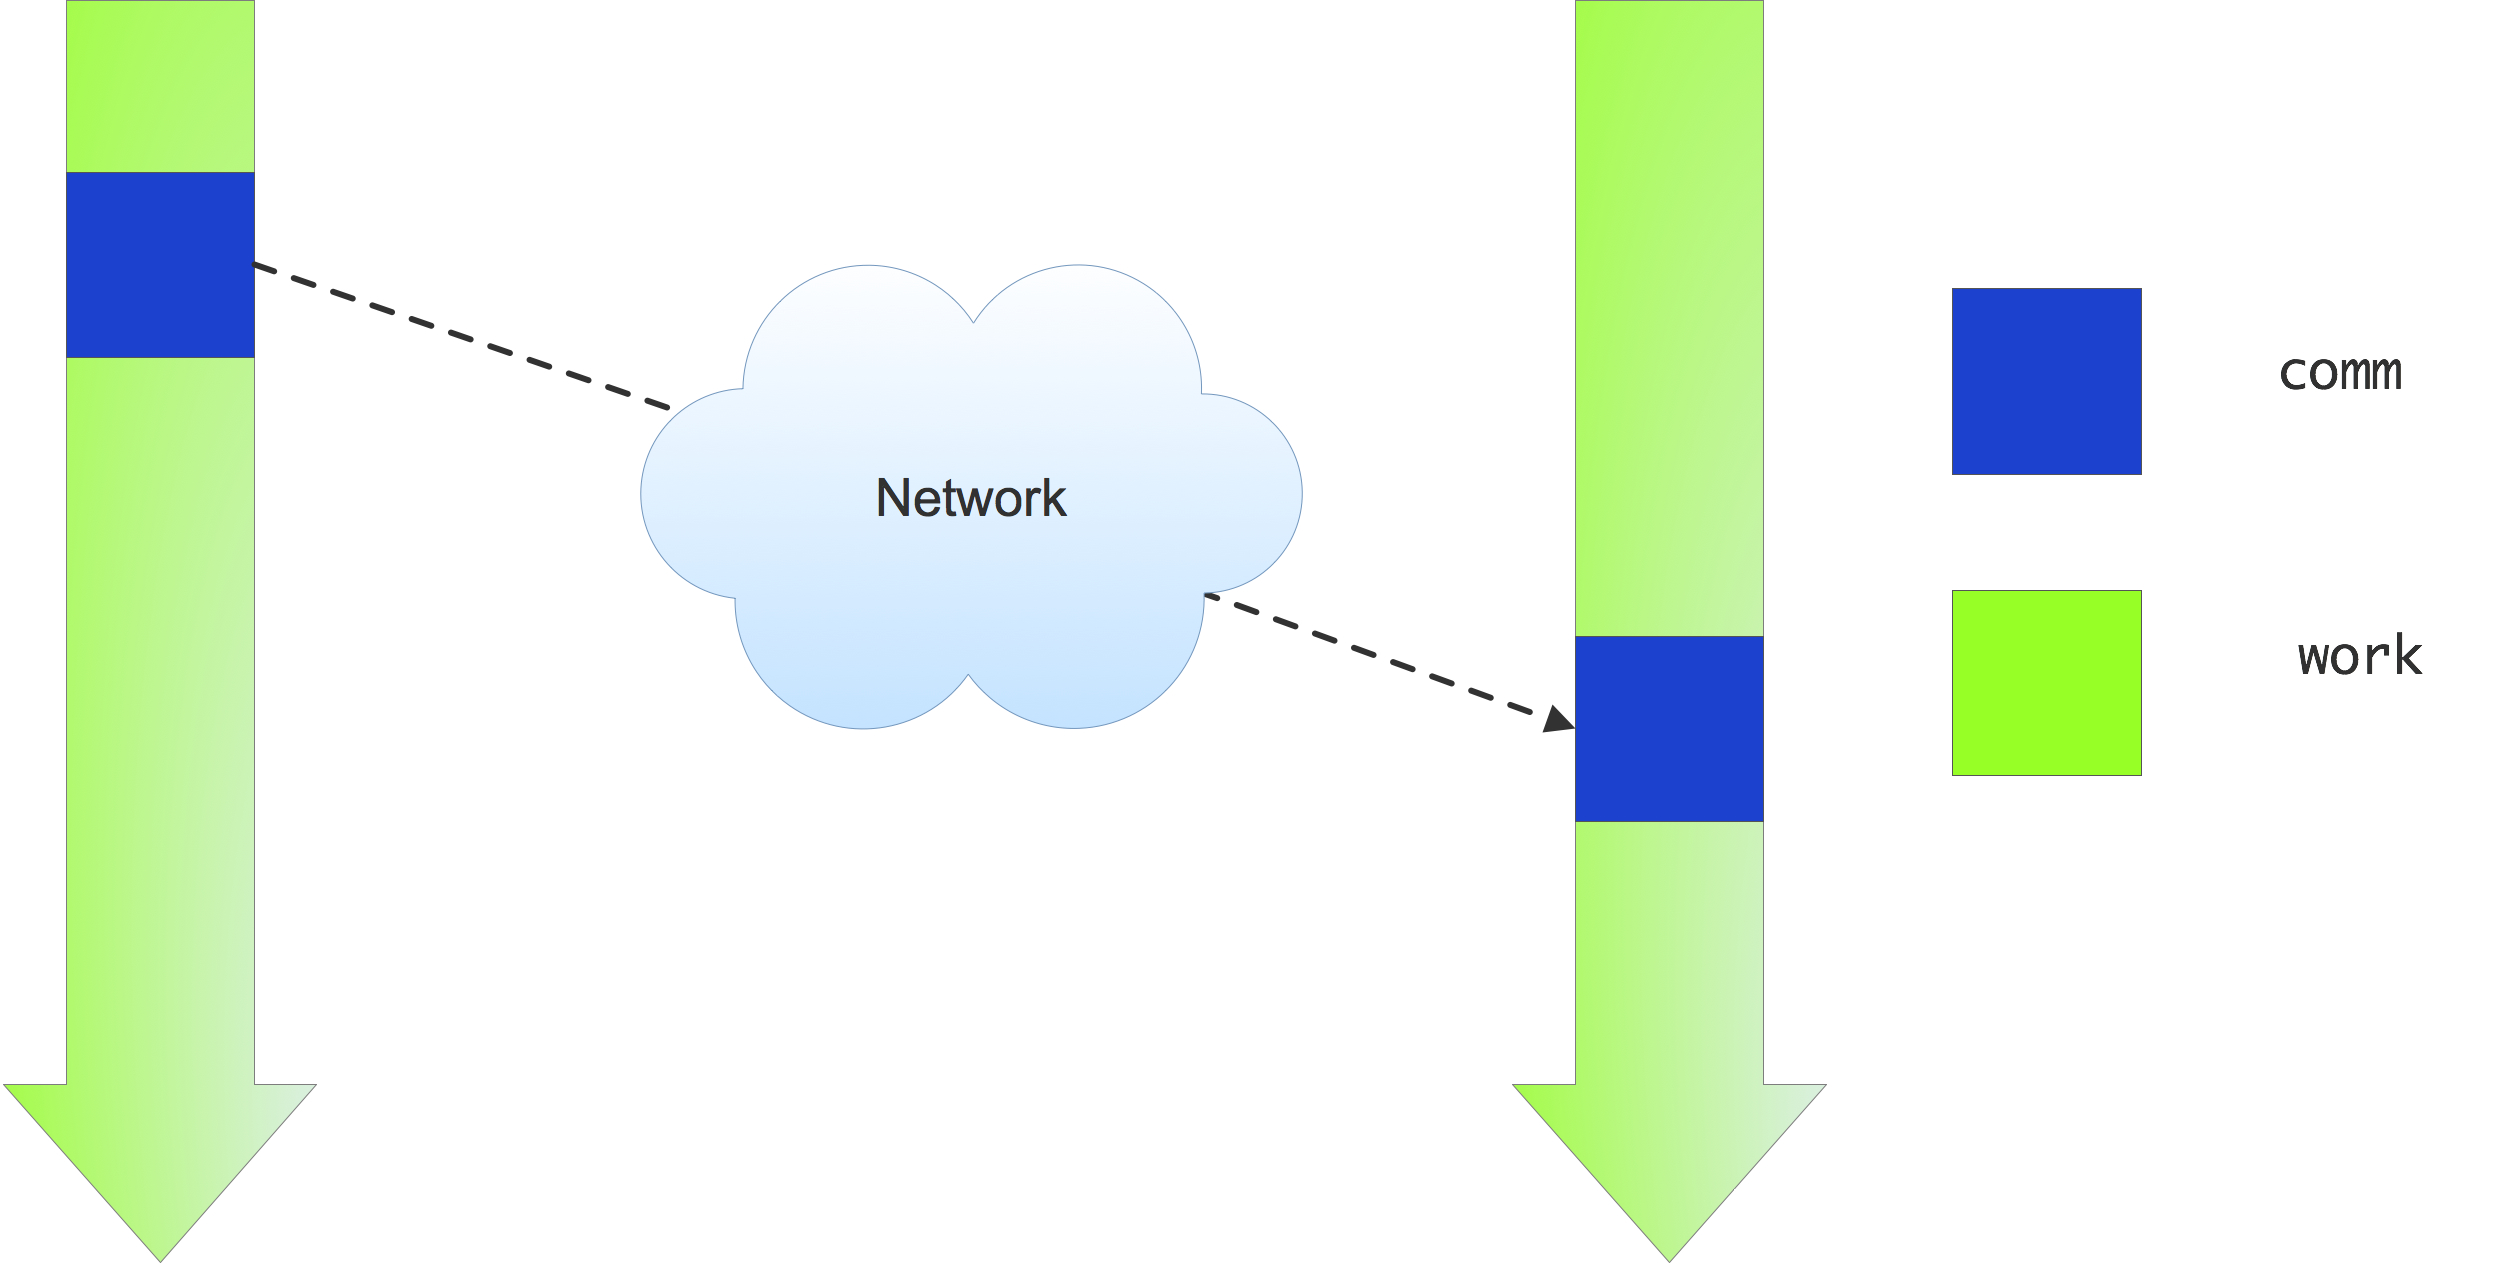
\includegraphics[scale=.08]{send-ideal}\hfill
  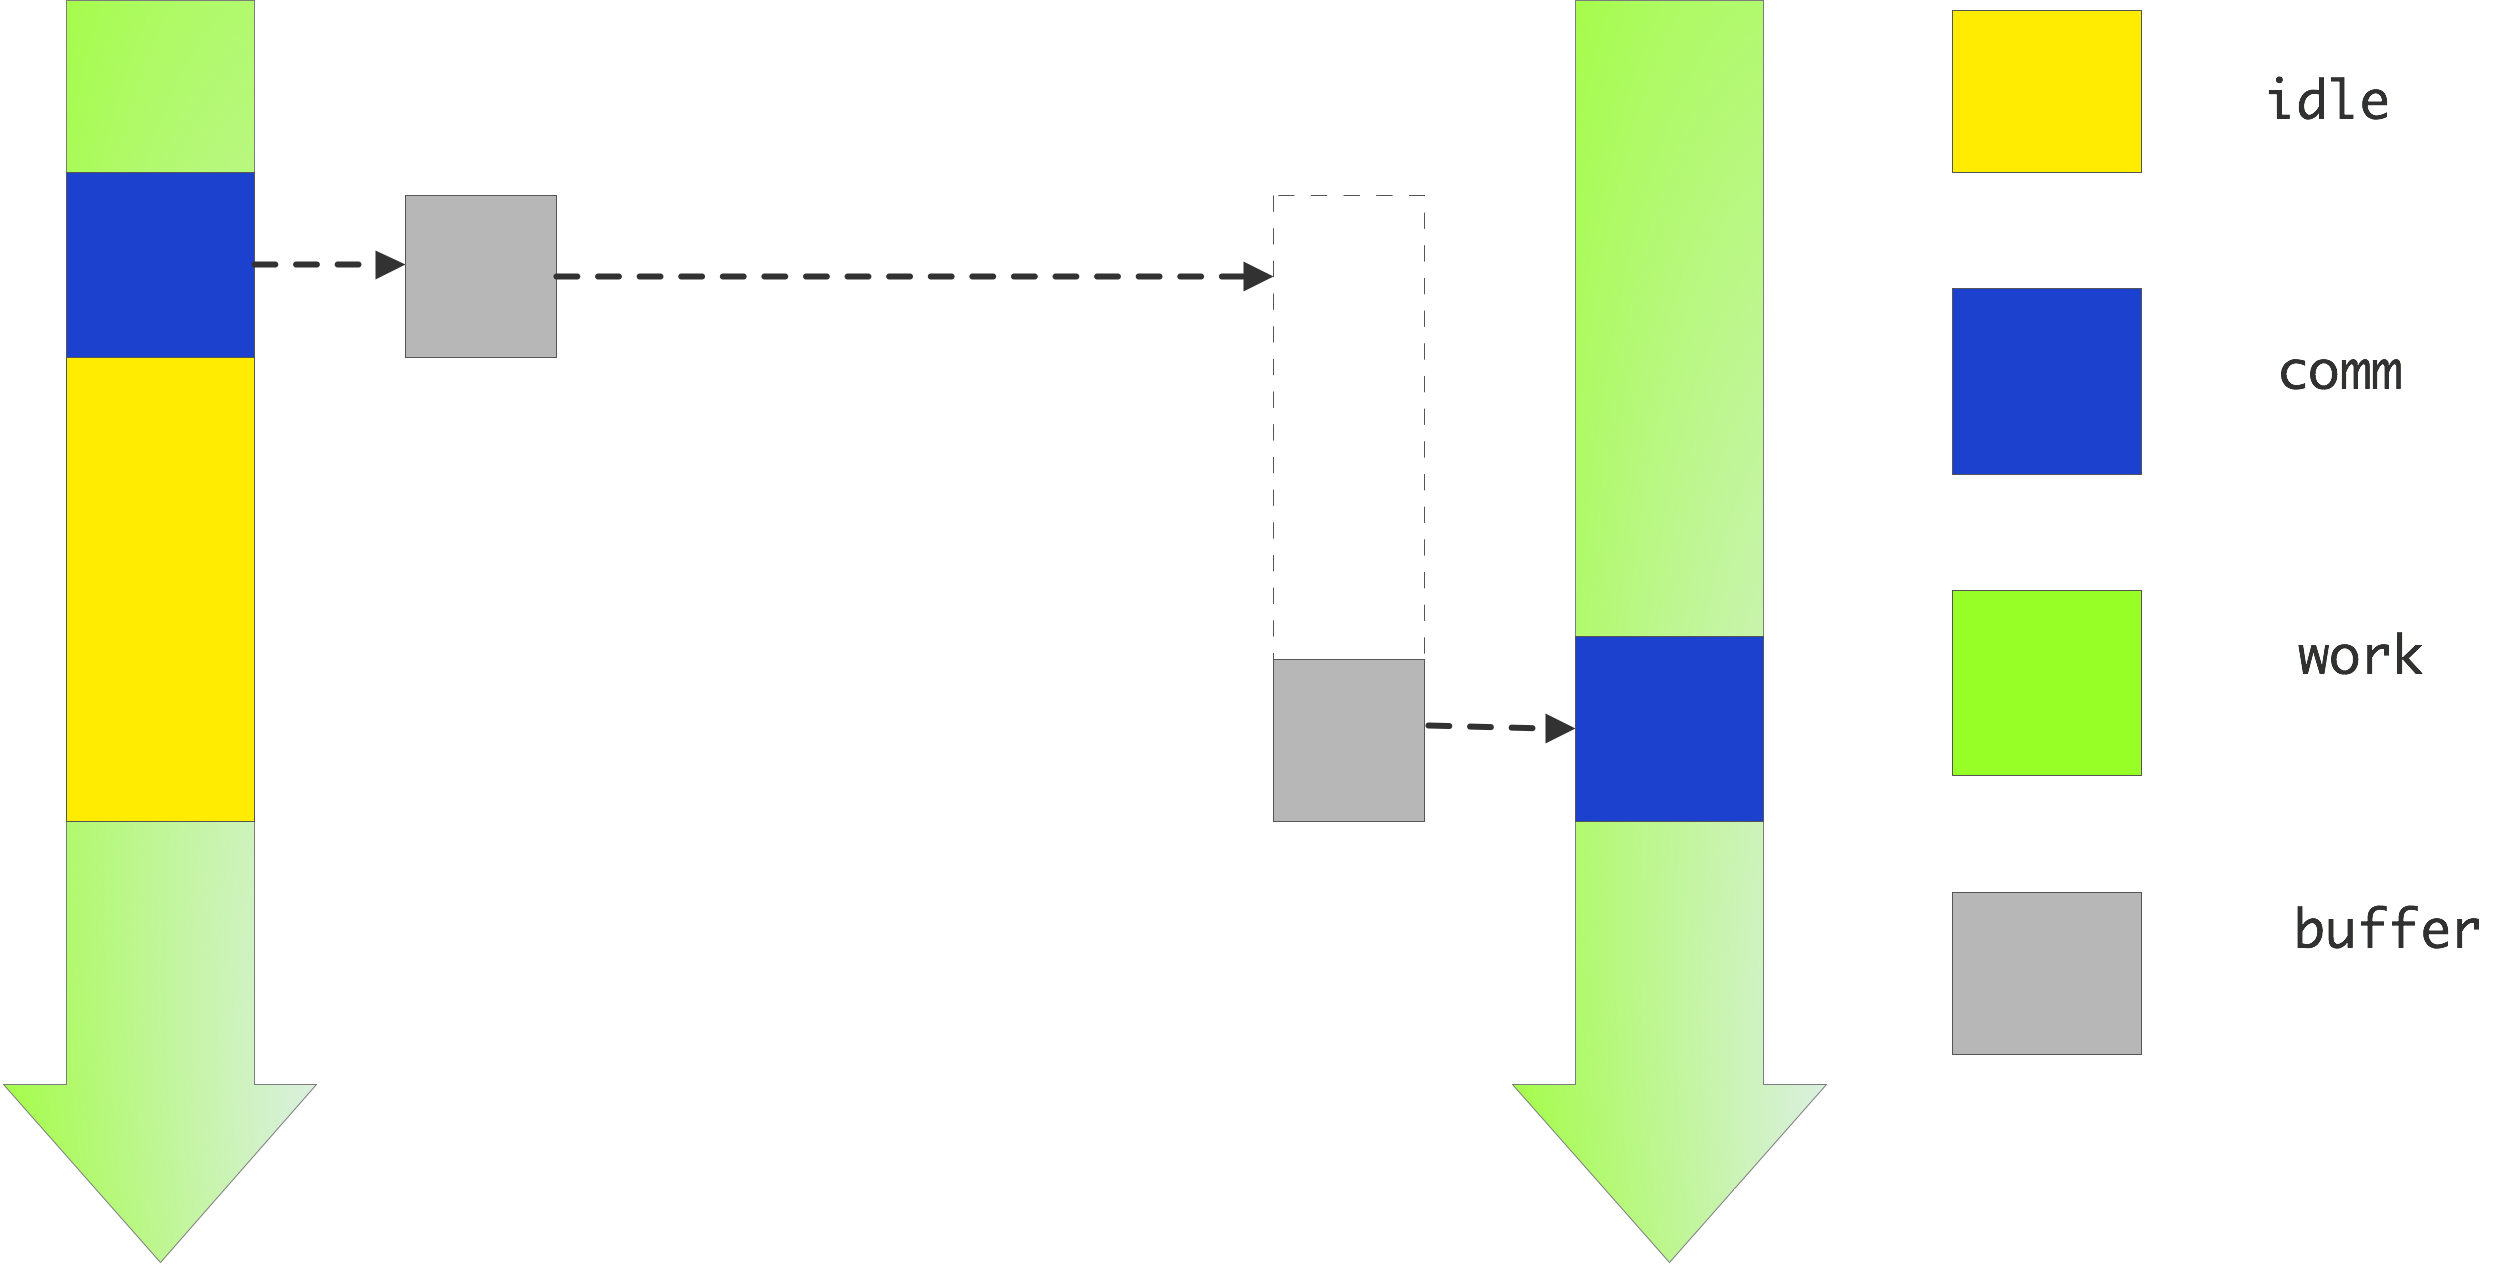
\includegraphics[scale=.08]{send-blocking}
  \caption{Illustration of `ideal' and `blocking' send}
  \label{fig:cw-send-blocking}
\end{figure}
This idealized behaviour is illustrated in the left half of
figure~\ref{fig:cw-send-blocking}. Practice is different.

Suppose a process sends a large message, something that takes
a great deal of memory. Since the only memory in the system
is on the processors, the message has to stay in the memory 
of one processor, until it is copied to the other.
We call this behaviour \indextermsub{blocking}{communication}:
a~send call will wait until the receiving processor is
indeed doing a receive call. That is, the sending code is blocked
until its message is received.

But this is a problem: if every process~$p$ starts sending to $p-1$,
everyone is waiting for someone else to do a receive, and no one is
actually doing a receive. This sort of situation is called
\indexterm{deadlock}.

\begin{exercise}
  Do you now see why the code fragment
  leads to deadlock? Can you come up with a clever rearrangement of the sends 
  and receives so that there is no deadlock?
\end{exercise}

Finding a `clever rearrangement' is usually not the best way to 
solve deadlock problems.
\begin{comment}
  One solution is to use \indextermsub{one-sided}{communication}.
  Here the idea is that:
  \begin{itemize}
  \item Each processor declares an area, called a `window', that is accessible to other
    pprocessors; and
  \item Other processors can then put data in another processor's window, or take data
    from it.
  \end{itemize}
  One-sided communication sounds attractive, but it is often easier and more efficient
\end{comment}
A common solution is
to use \indextermsub{non-blocking}{communication} calls. Here the send or receive instruction
only indicates to the system the buffer with send data, or in which to receive data. 
You then need a second call to ensure that the operation is actually completed.

In pseudo-code:
\begin{verbatim}
send( buffer1, to=neighbour1, result=request1 );
send( buffer2, to=neighbour2, result=request2 );
// maybe execute some other code
wait( request1 ); wait( request2 ); // make sure the operations are done
\end{verbatim}

\Level 2 {Task scheduling}
\label{sec:dag}

All parallel realizations of Life you have seen so far were based
on taking a single time step, and applying parallel computing to
the updates in that time step. This was based on the fact that
the points in the new time step can be computed independently.
But the outer iteration has to be done in that order. Right?

Well\ldots

Let's suppose you want to compute the board two timesteps from
now, without explicitly computing the next timestep. Would that be possible?

\begin{exercise}
  Life expresses the value in \n{i,j} at time $t+1$ as a simple
  function of the $3\times3$ patch \n{i-1:i+1,j-1:j+1} at time~$t$.
  Convince yourself that the value in \n{i,j} at~$t+\nobreak2$ can be
  computed as a function of a $5\times5$ patch at~$t$.

  Can you formulate rules for this update over two timesteps? Are
  these rules as elegant as the old ones, just expressed in a count of
  live and dead cells? If you would code the new rules as a case
  statement, how many clauses would there be? Let's not persue this
  further\ldots
\end{exercise}

This exercise makes an important point about dependence and
independence. If the value at \n{i,j} depends on
$3\times3$ previous points, and each of these have a similar
dependence, we can compute the value at \n{i,j} 
if we know $5\times5$ points two steps away, et cetera.
The conclusion is that you do not need to finish a whole time step before you 
can start the next: for each point update only certain other points
are needed, and not the whole board. If multiple processors are updating the board,
they do not need to be working on the same timestep.
This
is sometimes called \indexterm{asynchronous computing}.
It means that processors do not have to synchronize what time step they are working on:
within restrictions they can be working on different time steps.

\begin{exercise}
  Just how independent can processors be? If processor $i,j$ is
  working on time~$t$, can processor $i+1,j$ be working on $t+2$? Can
  you give a formal description of how far out of step processor $i,j$
  and $i',j'$ can be?
\end{exercise}

The previous sections were supposed to be about task parallelism, but
we didn't actually define the concept of task. Informally, a processor
receiving border information and then updating its local data sounds
like something that could be called a task.  To make it a little
more formal, we define a task as some operations done on the same
processor, plus a list of other tasks that have to be finished before
this task can be finished.

This concept of computing is also known as \indexterm{dataflow}: data
flows as output of one operation to another; an~operation can start
executing when all its inputs are available. Another concept connected
to this definition of tasks is that of a \acf{DAG}: the dependencies
between tasks form a graph, and you cannot have cycles in this graph,
otherwise you could never get started\ldots

You can interpret the MPI examples in terms of tasks.
The local computation of a task can start when data from the
neighbouring tasks is available, and a task finds out about that
by the messages from those neighbours coming in. However, 
this view does not add much information.

On the other hand, if you have shared memory, and tasks that do not
all take the same amount of running time, the task view can be
productive. In this case, we adopt a \indexterm{master-worker model}:
there is one master process that keeps a list of tasks, and there are
a number of worker processors that can execute the tasks. The master executes
the following program:
\begin{enumerate}
\item The master finds which running tasks are finished;
\item For each scheduled task, if it needs the data of a finished
  task, mark that the data is available;
\item Find a task that can now execute, find a processor for it, and
  execute it there.
\end{enumerate}
The pseudo-code for this is:
\begin{verbatim}
while there_are_tasks_left():
    for r in running_tasks:
        if r.finished():
            for t in scheduled_tasks:
                t.mark_available_input(r)
    t = find_available_task()
    p = find_available_processor()
    schedule(t,p)
\end{verbatim}

The master-worker model assumes that in general there are more
available tasks than processors. In the Game of Life we can easily get
this situation if you divide the board in more parts than there
are processing elements. (Why would you do that? This mostly makes
sense if you think about the memory hierarchy and cache sizes; see
section~\HPSCref{sec:hierarchy}.) So with
$N\times N$ divisions of the board and $T$~time steps, we define the queue
of tasks:
\begin{verbatim}
for t in [0:T]:
  for i in [0:N]:
    for j in [0:N]:
      task( id=[t+1,i,j], 
        prereqs=[ [t,i,j],[t,i-1,j],[t,i+1,j] # et cetera
                ] )
\end{verbatim}

\begin{exercise}
  Argue that this model mostly makes sense on shared memory. Hint: if
  you would execute this model on distributed memory, how much data
  needs to be moved in general when you start a task?
\end{exercise}

\Level 0 {Advanced topics}

\Level 1 {Data partitioning}
\label{sec:distribution}

The previous sections approached parallelization of the
Game of Life by taking the sequential implementation
and the basic loop structure. For instance, in
section~\ref{sec:mpi} we assigned a number of lines to each 
processor. This corresponds to a \indexterm{one-dimensional partitioning}
of the data.
Sometimes, however, it is a good idea to use a two-dimensional
one instead.
\begin{figure}[t]
  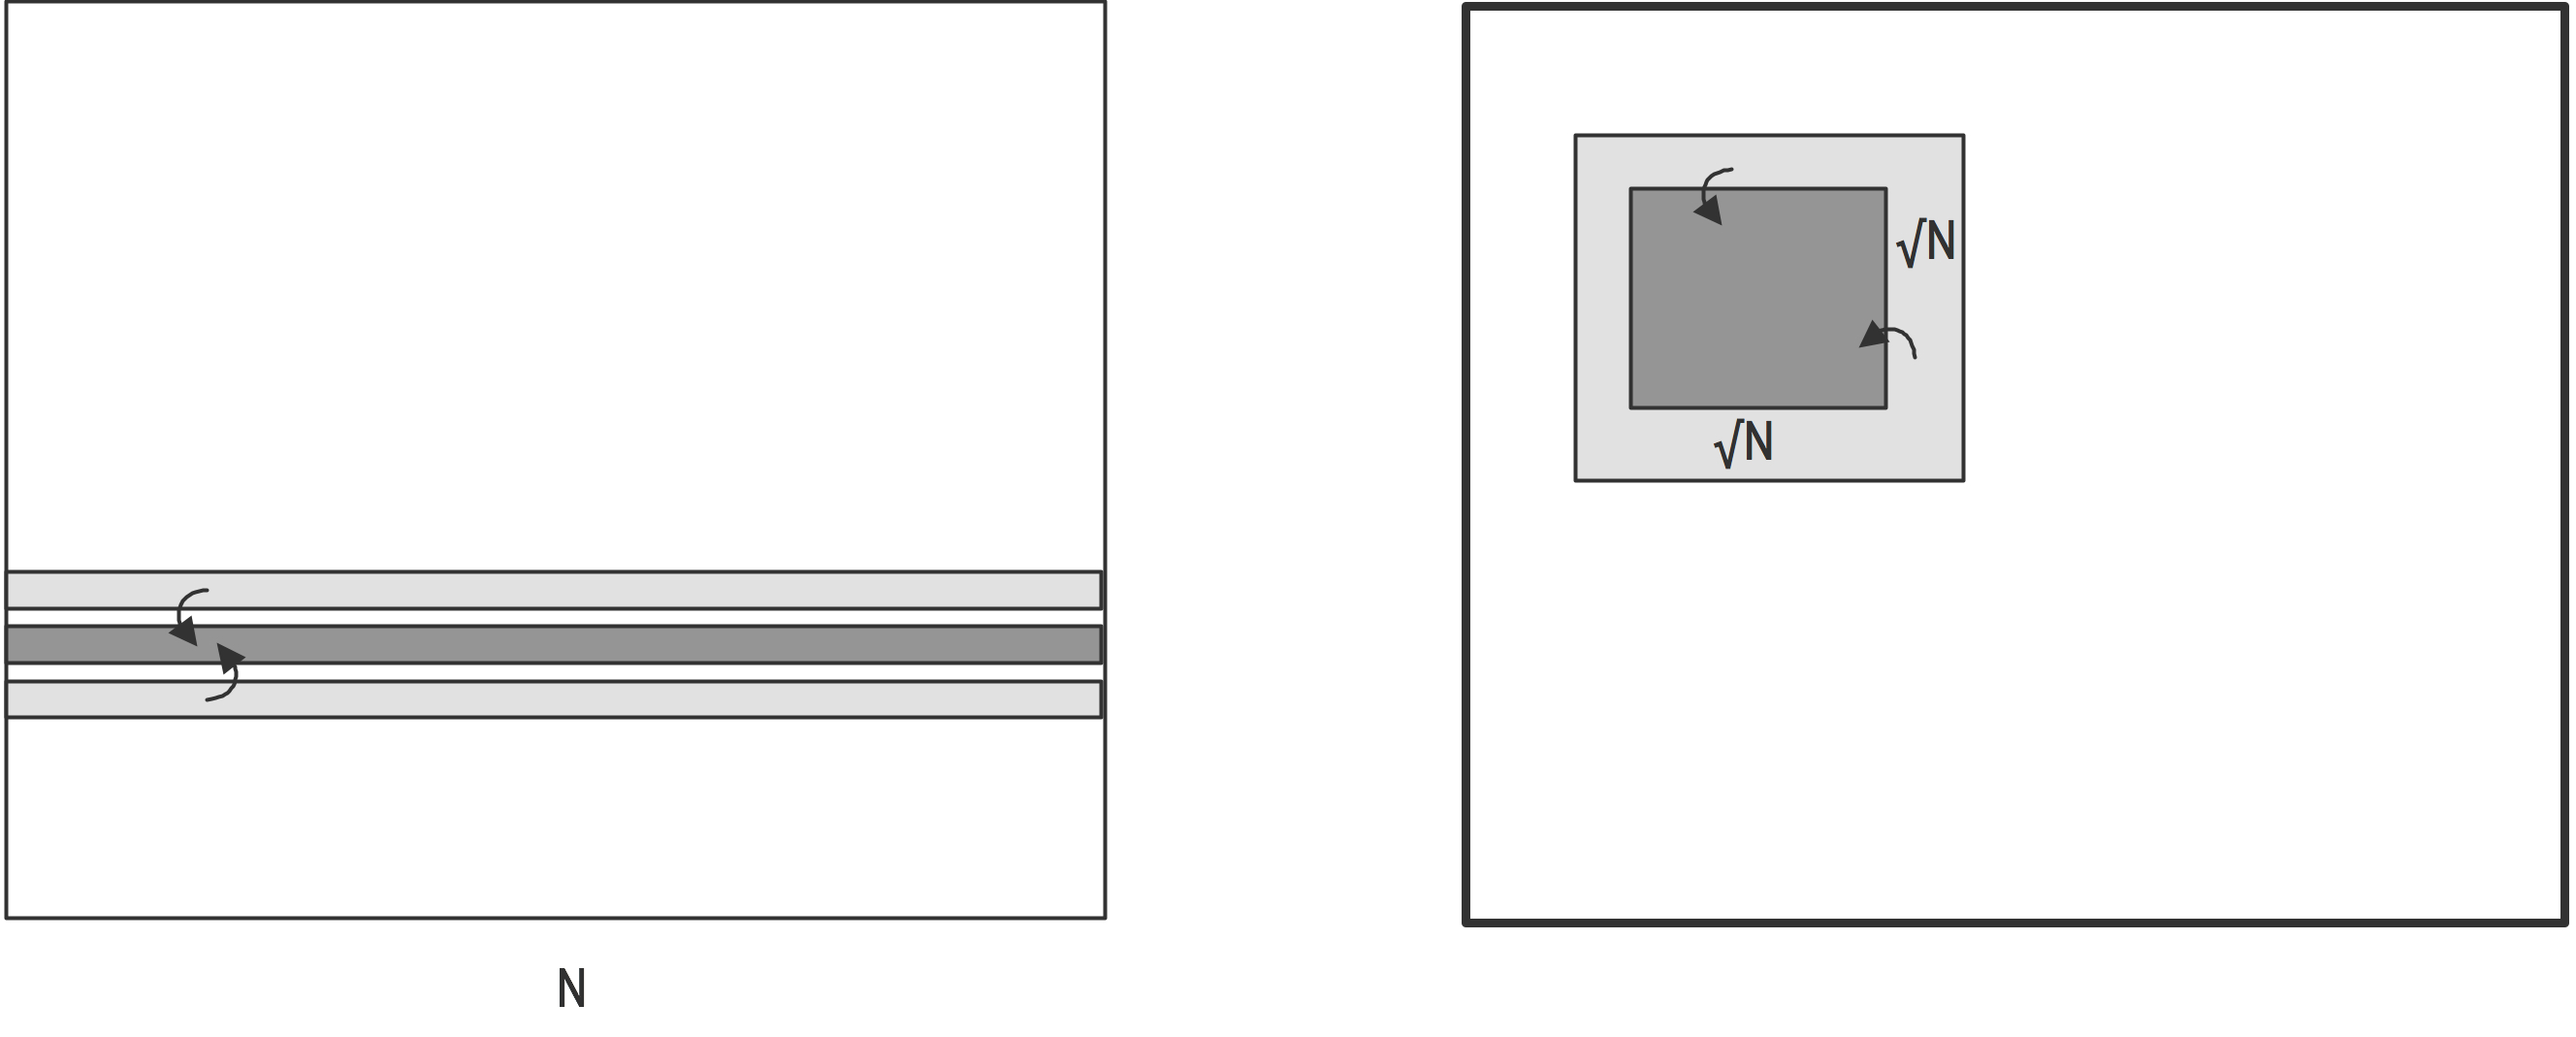
\includegraphics[scale=.15]{onetwod1}
  \caption{One-dimensional and two-dimensional distribution communication}
  \label{fig:onetwod1}
\end{figure}
(See figure~\ref{fig:onetwod1} for an illustration 
of the basic idea.) In this section you'll get the
flavour of the argument.

Suppose each processor stores one line of the Life board. 
As you saw in the previous section, to update that line it needs to receive
two lines worth of data, and this takes time.
In fact, receiving one item of data from another node is much slower
than reading one item from local memory. If we inventory the cost 
of one timestep in the distributed case, that comes down to
\begin{enumerate}
\item Receiving $2N$ Life cells from other processors\footnote{For now
  we only count the transmission cost per item; there is also a
  one-time cost for each transmission, called the \indexterm{latency}. For large enough messages we
  can ignore this; for details see~\HPSCref{sec:latencybandwidth}.}; and
\item Adding $8N$ values together to get the counts.
\end{enumerate}
For most architectures, the cost of sending and receiving data will
far outweigh the computation.

Let us now assume that we have $N$ processors, each storing a $\sqrt
N\times\sqrt N$ part of the Life board. We sometimes call this 
the processor's \indexterm{subdomain}.
To update this, a~processor
now needs to receive data from the lines above, under, and to the left
and right of its part (we are ignoring the edge of the board here).
That means four messages, each of size $\sqrt N+2$.
On the other hand, the update takes $8N$ operations. For large enough~$N$,
the communication, which is slow, will be outweighed by the computation,
which is much faster.

Our analysis here was very simple, based on having exactly~$N$ processors.
In practice you will have fewer processors, and each processor will
have a subdomain rather than a single point.
However, a more refined analysis gives the same conclusion:
a two-dimensional distribution is to be prefered over a one-dimensional one;
see for instance section~\HPSCref{sec:mvp-2d} for the analysis
of the matrix-vector product algorithm.

Let's do just a little analysis on the following scenario:
\begin{itemize}
\item You have a parallel machine where each processor has an amount
  $M$ of memory to store the Life board.
\item You can buy extra processors for this machine, thereby expanding
  both the processing power (in operations per second) and the total
  memory.
\item As you buy more processors, you can store a larger Life board:
  we're assuming that the amount $M$ of memory per processor is kept constant. (This
  strategy of scaling up the problem as you scale up the computer is
  called \indextermsub{weak}{scaling}. The scenario where you only
  increase the number of processors, keeping the problem fixed and
  therefore putting less and less Life cells on each processor,
  is called \indextermsub{strong}{scaling}.)
\end{itemize}

Let $P$ be the number of processors, and $N$ the size of the
board. In terms of the amount of memory $M$ you then have:
\[ M=N^2/P. \]

Let's now consider a one-dimensional distribution. (Left half of figure~\ref{fig:onetwod}.)
\begin{figure}[t]
  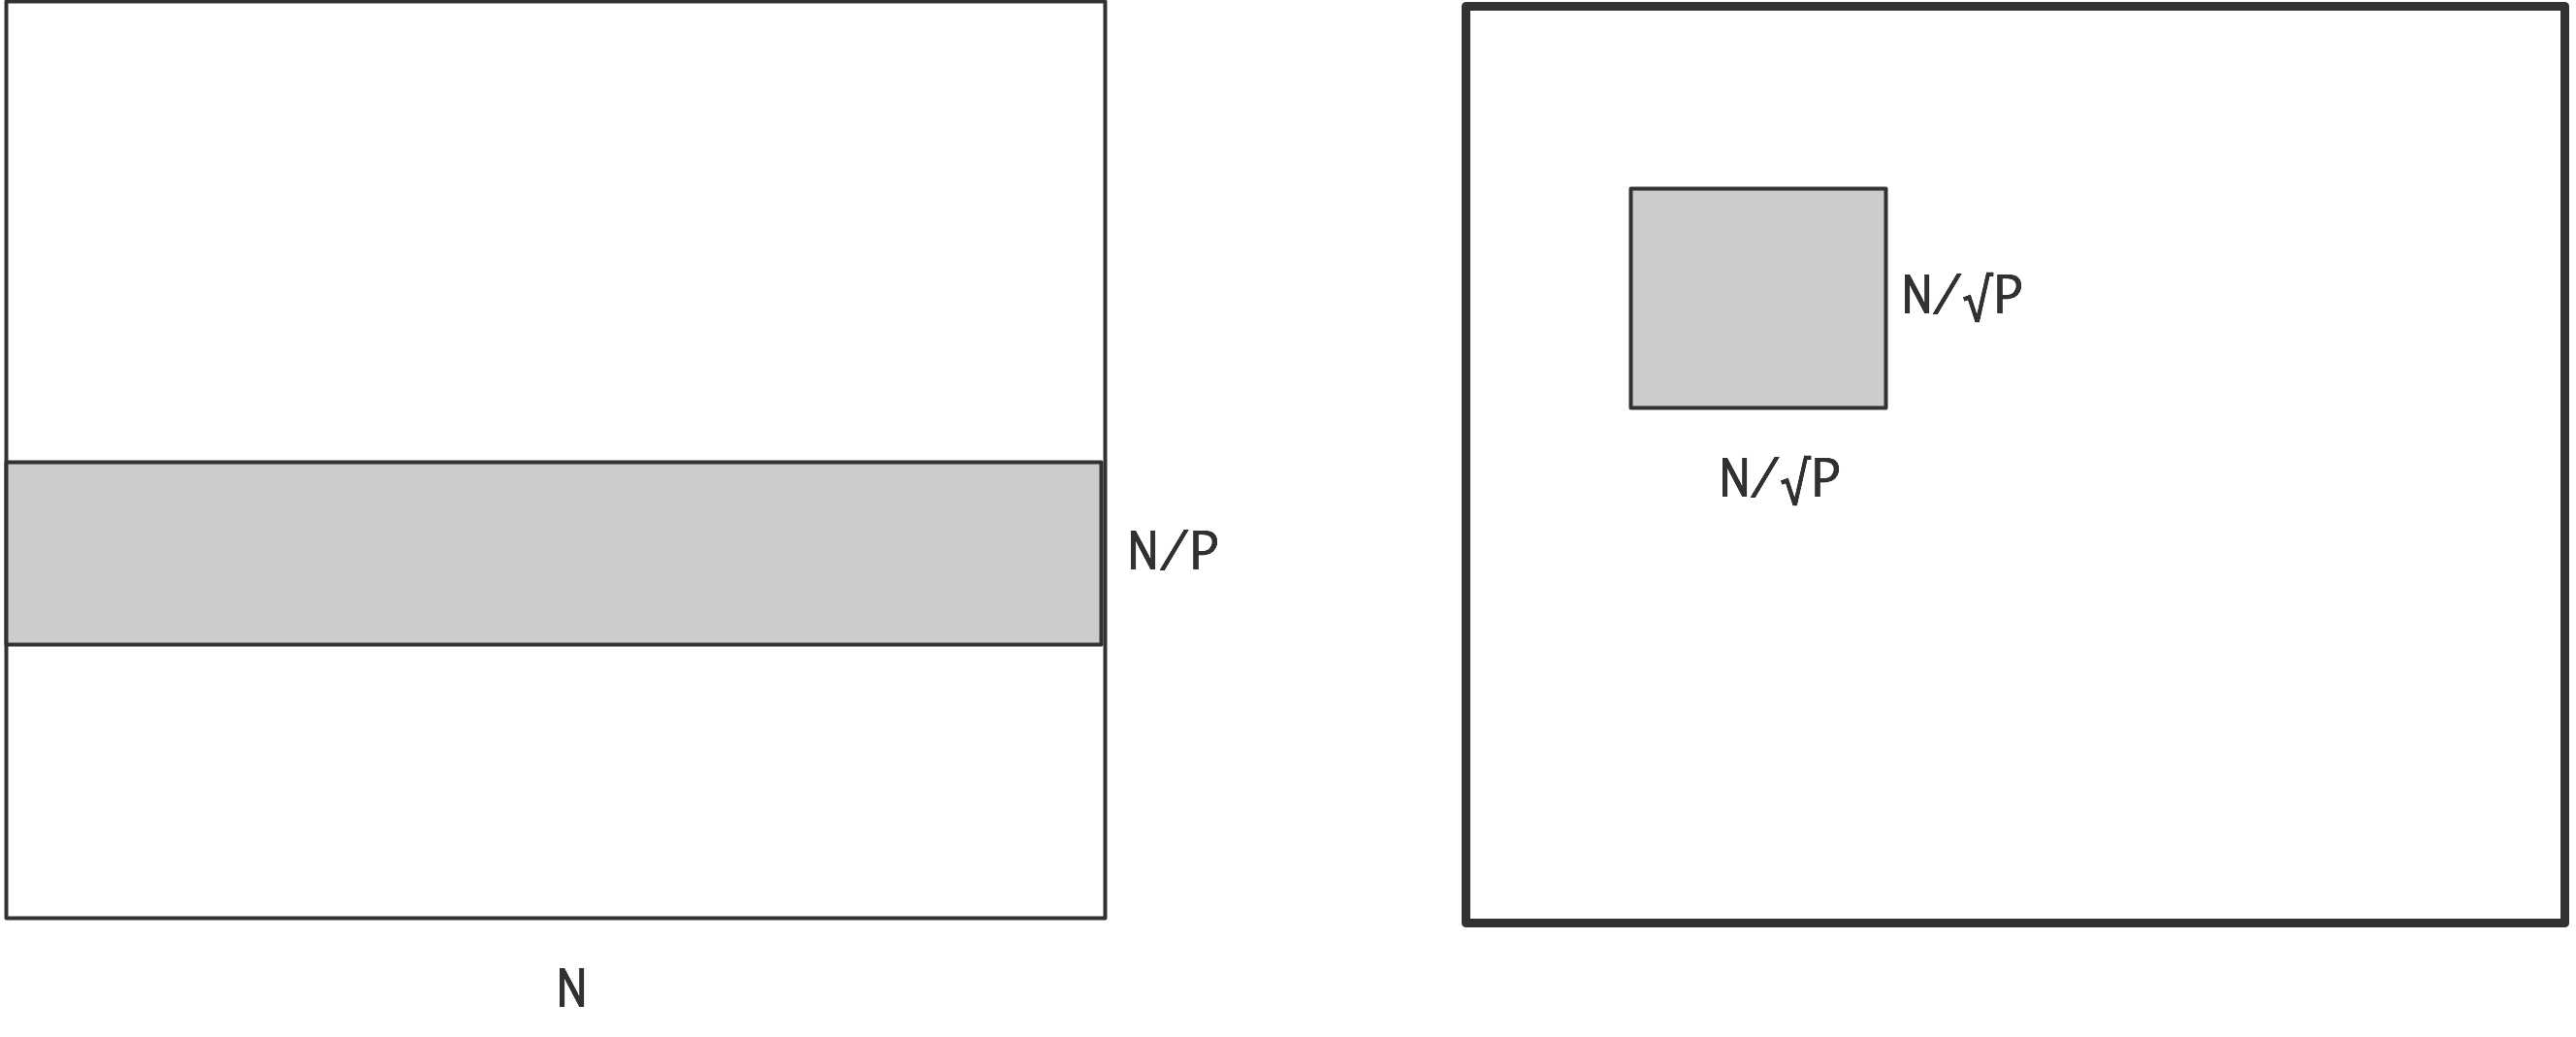
\includegraphics[scale=.15]{onetwod}
  \caption{One-dimensional and two-dimensional distribution of a Life board}
  \label{fig:onetwod}
\end{figure}
Every processor but
the first and last one needs to communicate two whole lines, meaning
$2N$ elements. If you express this in terms of $M$ you find a formula
that contains the variable~$P$. This means that as you buy more
processors, and can store a larger problem, the amount of
communication becomes a function of the number of processors.

\begin{exercise}
  Show that the amount of communication goes up with the number of
  processors. On the other hand, show that the amount of work stays
  constant, and that it corresponds to a perfect distribution of the
  work over the processors.
\end{exercise}

Now consider a two-dimensional distribution. (Right half of
figure~\ref{fig:onetwod}.)  Every processor that is not on the edge of
the board will communicate with eight others. With the four `corner'
processors only a single item is exchanged.

\begin{exercise}
  What is the amount of data exchanged with the processors left/right
  and top/bottom? Show that, expressed in terms of~$M$, this formula
  does not contain the variable~$P$. Show that, again, the work is
  constant in $N$ and~$P$.
\end{exercise}

The previous two exercises demonstrate an important point: different
parallelization strategies can have different overhead and therefore
different efficiencies. Both the
one and two-dimensional distribution lead to a perfect parallelization
of the work. On the other hand, with the two-dimension distribution
the communication is constant, while with the one-dimensional distribution
the communication cost goes up with the number of processors, so the
algorithm becomes less and less efficient.

\Level 1 {Combining work, minimizing communication}

In most of the above discussion we have considered the parallel update
of the Life board as one bulk operation that is executed in sequence:
you do all communication for one update step, and then the communication
for the next, et cetera.

Now, the time for a communication between two processes has two components:
there is a startup time (known as `latency'), and then there is a time
per item communicated. This is usually rendered as
\[ T(n) = \alpha+\beta\cdot n \]
where the $\alpha$ is the startup time and $\beta$~the per-item time.
 
\begin{exercise}
  Show that sending two messages of length~$n$ takes longer
  than one message of length~$2n$, in other words $T(2n)<2T(n)$.
  For what value of $n$ is the overhead~50\%? 10\%?
\end{exercise}

If the ratio between $\alpha$ and $\beta$ is large there is clearly
an incentive to combine messages. For the naive parallelization
strategies considered above there is no easy way to do this.
However, there is a way to communicate only once every \emph{two} 
updates. This communication will be larger, but there
will be savings in the startup cost.

\begin{figure}[t]
  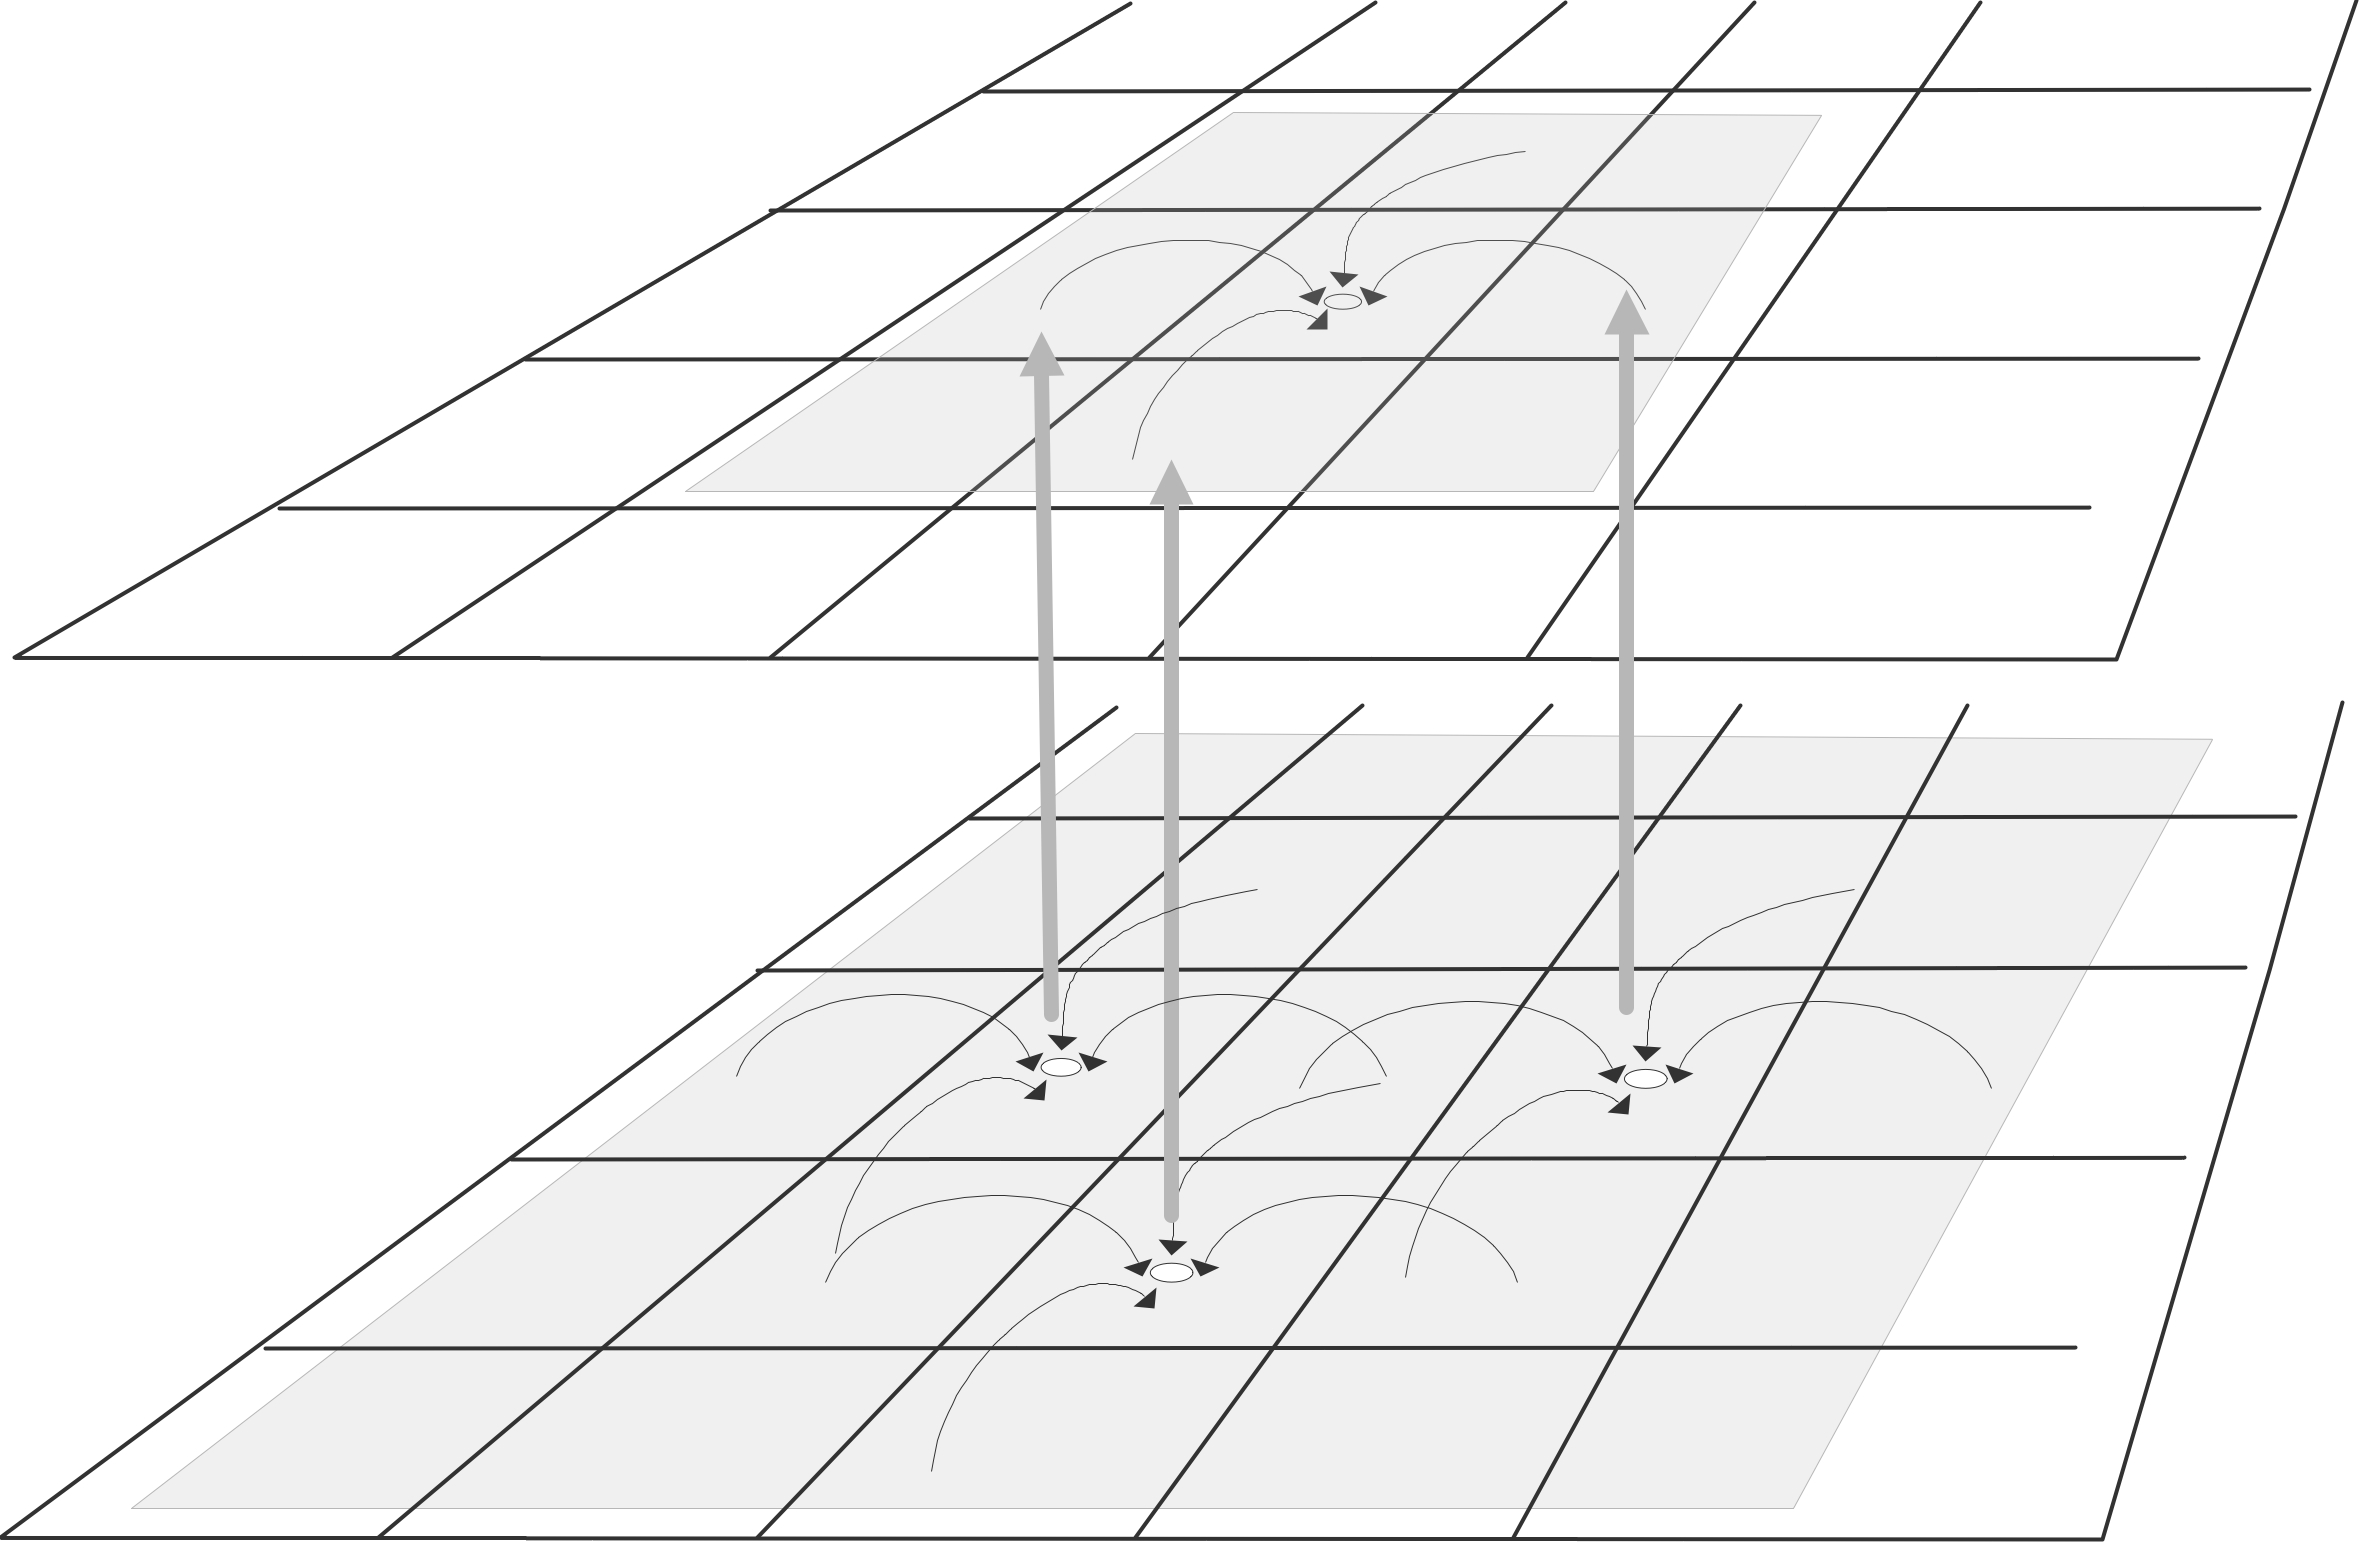
\includegraphics[scale=.15]{life-twostep}
  \caption{Two steps of Life updates}
  \label{fig:twostep}
\end{figure}

First we must observe that to update a single Life cell 
by one time step we need the eight cells around it. So to update
a cell by two time steps we need those eight cells plus the ones around them.
This is illustrated in figure~\ref{fig:twostep}.
If a processor has the responsibility for updating a subsection of the board,
it needs the \indexterm{halo region}
around it. For a single update, this is a halo of width~one, and
for two updates this is a halo of width~two.

Let's analyze the cost of this scheme. We assume that the board is
square of size $N\times N$, and that there are $P\times P$ processors,
so that each processor is computing an $(N/P)\times(N/P)$ part of the board.

In the one-step-at-a-time implementation a processor does the following:
\begin{enumerate}
\item Receives four messages of length $N$ and four of length~1; and
\item Then updates the part of the board it owns to the next time step.
\end{enumerate}
In order to update its subdomain two timesteps, the following is needed:
\begin{enumerate}
\item Receive four messages of size $2 N$ and four of size~4;
\item Compute the updated values at time~$t+1$ of the subdomain plus
  a locally stored border of thickness~1 around it;
\item Update precisely the owned subdomain to its state at~$t+2$.
\end{enumerate}
So now you send slightly more data, and you compute a little more,
but you save half the latency cost. Since communication latency can 
be quite high, this scheme can be faster overall.

\Level 1 {Load balancing}

The basic motivation of parallel computing is to be able to compute
faster.  Ideally, having $p$ processors would make your computation
$p$~times faster (see section~\HPSCref{sec:speedup-efficiency} for
definition and discussion of speedup), but practice doesn't always
live up to that ideal. There are many reasons for this, but one is
that the work may not be evenly divided between the processors.  If
some processors have more work than others, they will still be
computing while the others have finished and are sitting idle. This is
called \indexterm{load imbalance}.

\begin{exercise}
  Compute the speedup from using $p$ processors if one processor has a
  fraction $\epsilon$ more work than the others; the others are
  assumed to be perfectly balanced. Also compute the speedup from the
  case where one processor has $\epsilon$ less work than all
  others. Which of the two scenarios is worse?
\end{exercise}

Clearly, there is a strong incentive for having a well-balanced
load between the processors. How to do this depends on what sort
of parallelism you are dealing with.

In section~\ref{sec:dag} you saw that in shared memory it can make
sense to divide the work in more units than there are processors.
Statistically, this evens out the work balance.
On the other hand, in distributed memory (section~\ref{sec:mpi})
such dynamic assignment is not possible, so you have to be careful
in dividing up the work.
Unfortunately, sometimes the workload
changes during the run of a program, and you want to rebalance it.
Doing so can be tricky, since it requires problem data to be moved,
and processors have to reallocate and rearrange their data structures.
This is a very advanced topic, and not at all simple to do.

\endinput
\begin{review}
  \Level 1 {Review questions}
  \input review/conway
\end{review}
